\documentclass{article}



\usepackage{arxiv}

\usepackage[utf8]{inputenc} % allow utf-8 input
\usepackage[T1]{fontenc}    % use 8-bit T1 fonts
\usepackage{hyperref}       % hyperlinks
\usepackage{color}       % hyperlinks
\usepackage{url}            % simple URL typesetting
\usepackage{booktabs}       % professional-quality tables
\usepackage{amsfonts}       % blackboard math symbols
\usepackage{nicefrac}       % compact symbols for 1/2, etc.
\usepackage{microtype}      % microtypography
\usepackage{graphicx}

% Not in template
\usepackage{amsmath}
\usepackage{lineno}
\linenumbers

\newcommand{\RAN}[1]{{\color{blue}Richard: #1}}
\newcommand{\pierre}[1]{{\color{red}Pierre: #1}}

% \title{Seasonal influenza: the limits of predictability}
% \title{Limited predictability of seasonal influenza virus evolution}
\title{Limited predictability of clade frequencies of seasonal influenza viruses}

%\date{September 9, 1985}	% Here you can change the date presented in the paper title
\date{} 					% Or removing it

\author{Pierre Barrat-Charlaix\\
	Biozentrum\\
	Univeristät Basel\\
	Basel, Switzerland \\
	\texttt{pierre.barrat@unibas.ch} \\
	% %% examples of more authors
	\And
	\hspace{1mm}Richard Neher \\
	Biozentrum\\
	Univeristät Basel\\
	Basel, Switzerland \\
	\texttt{richard.neher@unibas.ch} \\
}

\begin{document}
\maketitle

\begin{abstract}
    \RAN{the abstract needs streamlining -- I can take a crack once the ms is stable}
	Seasonal influenza viruses causes a major epidemic every year in the human population, while mutating rapidly to evade host immune systems. Predicting which mutations will fix in its genome is of course critical to developing a vaccine, but also challenges our ability to understand the underlying evolutionary dynamics driving them. In this work, we use sequences of the influenza hemagglutinin (HA) from the last 20 years to assess our ability to predict the outcome of mutations in the virus\'s genome. Investigating the frequency trajectories of new amino acid mutations and their probability to fix in the flu population, we failed to find signatures of selection. On the contrary, our results differ little from a scenario of neutral evolution, implying strong limits to predictability. Interestingly, looking at known antigenic positions in HA or using proxies for fitness such as the \emph{Local Branching Index} (LBI) changes very little to these results, whereas the geographical spread or the age of a mutation are found to be informative of its probability to fix in the population. Finally, we try to find reasons for the predictive success of quantities such as the LBI. In doing so, we show the simple method of taking the consensus sequence of the current flu population fares slightly but consistently better than the LBI. Overall, our results indicate that the evolution of HA sequences happens in an unintuitive manner and does not agree with predictions of usual models such as travelling fitness waves.  
\end{abstract}

\section*{Introduction} % (fold)
\label{sec:introduction}
	
	Seasonal influenza A viruses (IAV) infect on the order of 10\% of the global population every year, resulting in hundreds of thousands of deaths~\cite{WHOfactsheet,petrova_evolution_2017}. Vaccination is primary measure to reduce influenza morbidity and the World Health Organization (WHO) regularly updates influenza vaccine recommendations to best match the circulating strains. However, the long time needed to develop and produce vaccines combined with the rapid antigenic evolution of influenza strains makes keeping the vaccine up to date a challenging task. Indeed, the surface proteins hemagglutinin (HA) and neuraminidase (NA) continuously accumulate mutations at a fast rate, leading to frequent antigenic changes \cite{petrova_evolution_2017, Shih6283, koelle2009understanding}. While a vaccine targeting a particular antigenic subtype may be efficient for some time, antigenic drift will sooner or later render it obsolete. This makes our ability to forecast the evolution of influenza of essential interest to public health. \\
	Over the last 20 years, sequencing efforts and better sequence sharing possibilities have resulted in an exponential increase in the availability of high quality HA and NA sequences~\cite{bogner2006global, shu2017gisaid}. This has made possible the analysis of sequence evolution at a fine temporal scale, resulting in a rich field of viral evolution prediction models~\cite{morris2018predictive}. These models aim at predicting the future population of influenza viruses based on estimations of the current fitness of strains. Fitness has been estimated by a variety different approaches, all showing a degree of success. In \cite{luksza_predictive_2014}, a sequence fitness model capturing antigenic drift and protein stability is trained using epitope and non-epitope mutations. Another approach in \cite{Steinbrueck12123} relies on hemagglutination inhibition (HI) assays to determine possible antigenic shifts for clades in the genealogy of the HA protein. Finally, \cite{neher_predicting_2014} uses the dense branching of HA genealogy as a growth measure. \\
	The underlying assumption of all these methods is that some mutations in surface proteins are under a strong positive selection, especially those responsible for antigenic drift, and thus rapidly fix in the population. In this work, we use sequences from HA and NA proteins in H3N2 influenza from year 2000 to 2019 to perform a retrospective analysis of frequency trajectories of amino acid mutations. The question we ask is whether the selective pressure for new antigenic properties confers, on average, a typical shape to frequency trajectories of amino acid mutations, and whether this could be used to predict their future. To our surprise, we find that the predictability of these trajectories is very limited. Indeed, many of their properties seem compatible with selective neutrality, even in epitope positions. This observation is not attributable solely to clonal interference and genetic linkage, as simple simulations including those effects fail to reproduce it. In coherence with these observations, we show that a simple predictor uninformed about fitness, the consensus sequence, performs as the well as the Local Branching Index (LBI), the growth measure based on the genealogy used in \cite{neher_predicting_2014}. This suggests that although LBI has some predictive power, the reason for its success may not be related to it approximating fitness of strains.  

% section introduction (end)


\section*{Results} % (fold)
\label{sec:results}

	The main underlying question asked in this work is the following: given a mutation $X$ in the genome of H3N2 influenza that we observe at a frequency $f$ in the population at a given date, what can we say about the future of $X$?  \\
	There are different ways to make this question more specific. First, one can try to quantitatively predict the frequency of $X$ at future times $f(t)$. In other words, having observed a mutation at frequencies $(f_1, f_2,\ldots,f_n)$ at dates $(t_1,t_2,\ldots,t_n)$, what can we say about its frequency at future dates $(t_{n+1}, t_{n+2},\ldots)$? %In figure \ref{fig:panel2} (bottom part), this amounts to predicting the shape of the frequency trajectory curves after the date indicated by a vertical line using all past information. 
	This type of prediction will be referred to as \emph{short term}.  \\
	Another way to formulate this question is to ask whether $X$ will fix in the population, will disappear, or will stay as a polymorphism. Here, fixation is meant as reaching a dominant frequency in the population for a long enough period of time (see Methods). Since many mutations define a clade in the phylogenetic tree of influenza, this amounts to asking which of these clades will be the ancestor of the future flu population, a question of critical importance for vaccine design. It will be referred to in the following as a \emph{long term prediction}.

	% \begin{figure}
	% 	\centering
	% 	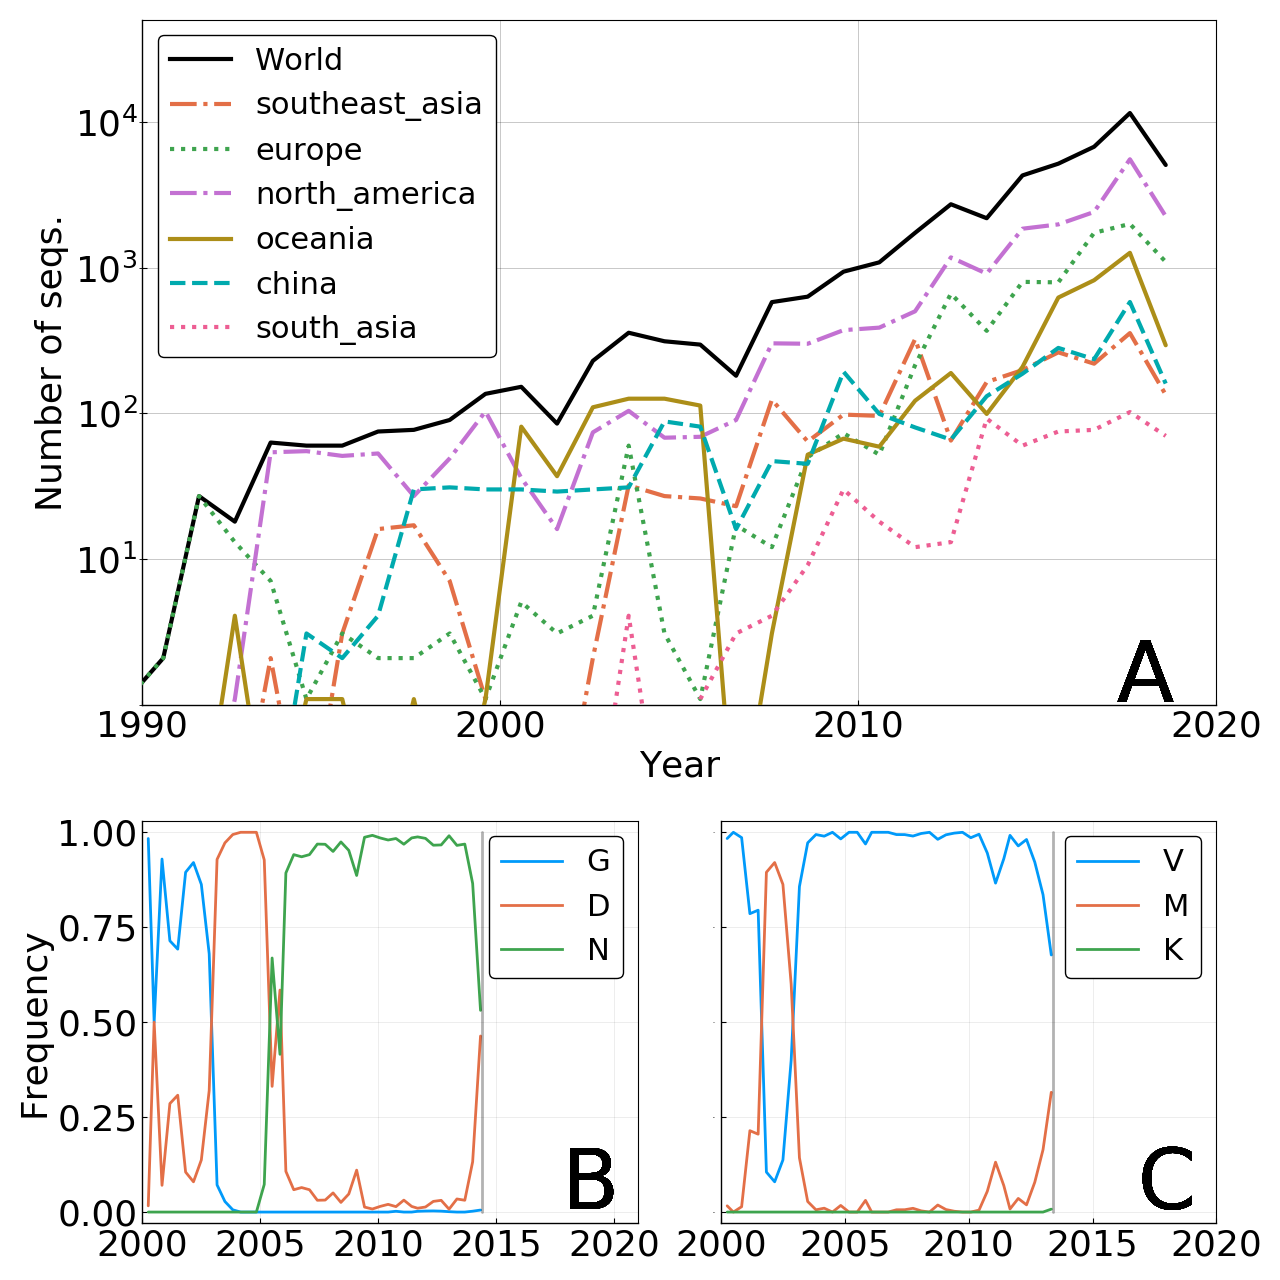
\includegraphics[width=0.9\textwidth]{Figures/Panel1.png}
	% 	\caption{}
	% 	\label{fig:panel1}
	% \end{figure}

	In this work, we use all publicly available amino-acid sequences of the HA and NA genes of H3N2 influenza since the year 2000. This amounts to $44\,976$ HA and $36\,300$ NA sequences, with a minimum of 100 per year. These sequences are binned in non-overlapping intervals of one month. Each single-month time bin and the sequences that it contains represents a snapshot of the H3N2 population at a given date. The number of sequences per time bin varies strongly both with year and according to the season, with earlier time bins containing around 10 sequences while more recent bins contain several hundreds (see figures~\ref{fig:nseq_per_year} and \ref{fig:nseq_per_month} in SM for details).\\
	The central quantities that are derived from this data are \emph{frequency trajectories} of amino acids at each position in the sequences. If an amino acid $X_i$ is found at position $i$ at a frequency between 5\% and 95\% in the population of a given time bin $t$, then the population is considered polymorphic at position $i$ and at time $t$. This polymorphism is characterized by the frequency of $X_i$, $f_{X_i}(t)$, and also by frequencies of other amino acids at $i$. The series of values $f_{X_i}(t)$ for contiguous time bins constitutes the frequency trajectory of $X_i$. A trajectory is terminated if the corresponding frequency is measured above 95\% (resp. below 5\%) for two time bins in a row, in which case amino acid $X_i$ is considered as \emph{fixed} (resp. \emph{absent}) in the population. Otherwise, the trajectory is considered \emph{active}. Examples of trajectories can be seen in figure~\ref{fig:sample_trajectories} of the Supplement.\\% [NOTE: I also explain this in Methods. Maybe shorten this part]\\
	Frequency trajectories allow a simple formulation of the above-stated questions. The short term prediction amounts to predicting the curve $f(t)$ starting from a given date $t_0$. On the other hand, the long term prediction amounts to predicting how long a trajectory will remain active, and whether it will fix or disappear when it finishes. \\
	In the rest of this work, we will focus on frequency trajectories that are starting at a null frequency, \emph{i.e.} $f(t=0)=0$. These represent new amino acid mutations which were absent in the past and are currently rising in the population. Two reasons motivate this. The first is simply that this avoids the problem of non-independent trajectories. Indeed, each rising trajectory implies the existence of another decreasing one at the same position, since frequencies of all amino acids at a given position must sum to one. By considering new mutations only, we restrict ourselves to independent trajectories. \\
	The second is that we expect to see a stronger signal of selection for this type of mutations. Current research on influenza seems to indicate that surface proteins HA and NA are under strong selective pressure as they have to escape hosts immune systems. This escape is driven by adaptive mutations, for instance on epitopes of the mentioned proteins. For this reason, one could expect new amino acid mutations that have reached a high enough frequency to be on average \emph{positively} selected, and their frequency trajectories should reflect this by showing a regular increase until they take over the population. We will call such a change in the dominant amino acid at a position a \emph{sweep}, examples of which can be seen in some trajectories represented in supplementary figure~\ref{fig:sample_trajectories}. By restricting ourselves to trajectories that start at low frequency, we should bias the mutations we analyse towards positively selected ones, thus making them easier to predict as well as recovering a clearer signal of selection. \\

	Sequences are also used to build a phylogenetic tree of HA and NA genes. For computational reasons, the number of sequences used to infer the tree is limited to 100 per 4 months (randomly chosen), totalling 4402 sequences over the 2000-2019 time period. The inference is done using the \emph{iqtree} software with default settings~\cite{10.1093/molbev/msaa015,10.1093/molbev/msu300}. \\

	\subsection*{Short term prediction}

	Having observed the frequency trajectory $f(t)$ of a mutation until a given date $t_0$, how much can we say about the future values of $f$ after $t_0$? To make the question more specific, we consider the idealized case sketched on panel \textbf{A} of figure~\ref{fig:panel2}: given the trajectory of a \emph{new} mutation, \emph{i.e.} that started at a frequency of 0, and that we observe at frequency $f_0$ at time $t_0$, what is the probability $P_{\Delta t}(f)$ of observing it at a value $f$ at time $t_0 + \Delta t$? \\
	To answer this question retrospectively, we use all frequency trajectories extracted from HA H3N2 sequences that satisfy these conditions for a given $f_0$. Since actual frequency trajectories rely on a finite number of sequences, we cannot exactly measure them at a precise frequency $f_0$. For this reason, we allow some leeway around $f_0$, considering all trajectories measured in the interval $[f_0-\delta f, f_0+\delta f]$ with $\delta f = 0.05$. \\
	For $f_0=0.3$, we find 69 such trajectories, represented on the panel \textbf{B} of figure~\ref{fig:panel2}, where time is shifted such that $t_0 =0$. It can be noted that some of those trajectories fall in the frequency bin around $f_0$ while decreasing, even though they crossed that bin at an earlier time. This again comes from the fact that frequencies are based on a finite number of sequences, resulting in some trajectories being measured below the selected frequency bin at a given time bin and above it at the next time bin. These trajectories are nevertheless rising in the sense that they start at frequency 0 for $t\rightarrow -\infty$. Removing them does not change results significantly. \\
	Since influenza is often thought of as permanently evading the human immune system, one could expect that a significant fraction of new amino acid mutations that have reached a finite frequency represented by rising trajectories on figure~\ref{fig:panel2} are \emph{adaptive} mutations under positive selection. We could thus expect that most of these trajectories continue rising after reaching frequency $f_0$ in an "inertial" manner, at least for some short enough amount of time. A fraction of those would then sweep through the population and smoothly reach a dominant frequency or fix. \\
	Trajectories collected and shown in figure~\ref{fig:panel2} are used to verify if past trajectories did behave in this inertial manner, and to measure the corresponding "persistence time", that is the amount of time during which the trajectory will keep rising. In practice, we  estimate the probability distribution $P_{\Delta t}(f)$ of finding a trajectory at frequency $f$ after a time $\Delta t$. Results are shown on panel \textbf{C} of figure~\ref{fig:panel2}. Initially, \emph{i.e.} at time $t_0=0$, this distribution is by construction peaked around $f_0$. If a large fraction of the trajectories keep increasing after this time, we should see the "mass" of $P_{\Delta t}(f)$ move to the right towards higher frequencies as time progresses.\\
	 However, future distributions for $\Delta t >0$ do not seem to behave according to this hypothesis. Indeed, our results show that the frequency distribution seems to  flatten more or less symmetrically in the first 30 to 60 days. After longer times of a year to two years, if we exclude mutations that have disappeared or fixed, this distribution becomes almost flat (leftmost and rightmost bins of the distribution). This indicates that what we called the persistence time of frequency trajectories is rather small, of the order of a month at most. After a few months, knowledge that the trajectory was rising and arriving at frequency $f_0$ is mostly lost. This contradicts the view that influenza's evolution is dominated by adaptive sweeps which take over the population and suggests a strong limit to our ability to predict the future of frequency trajectories.  

	\begin{figure}
		\centering
		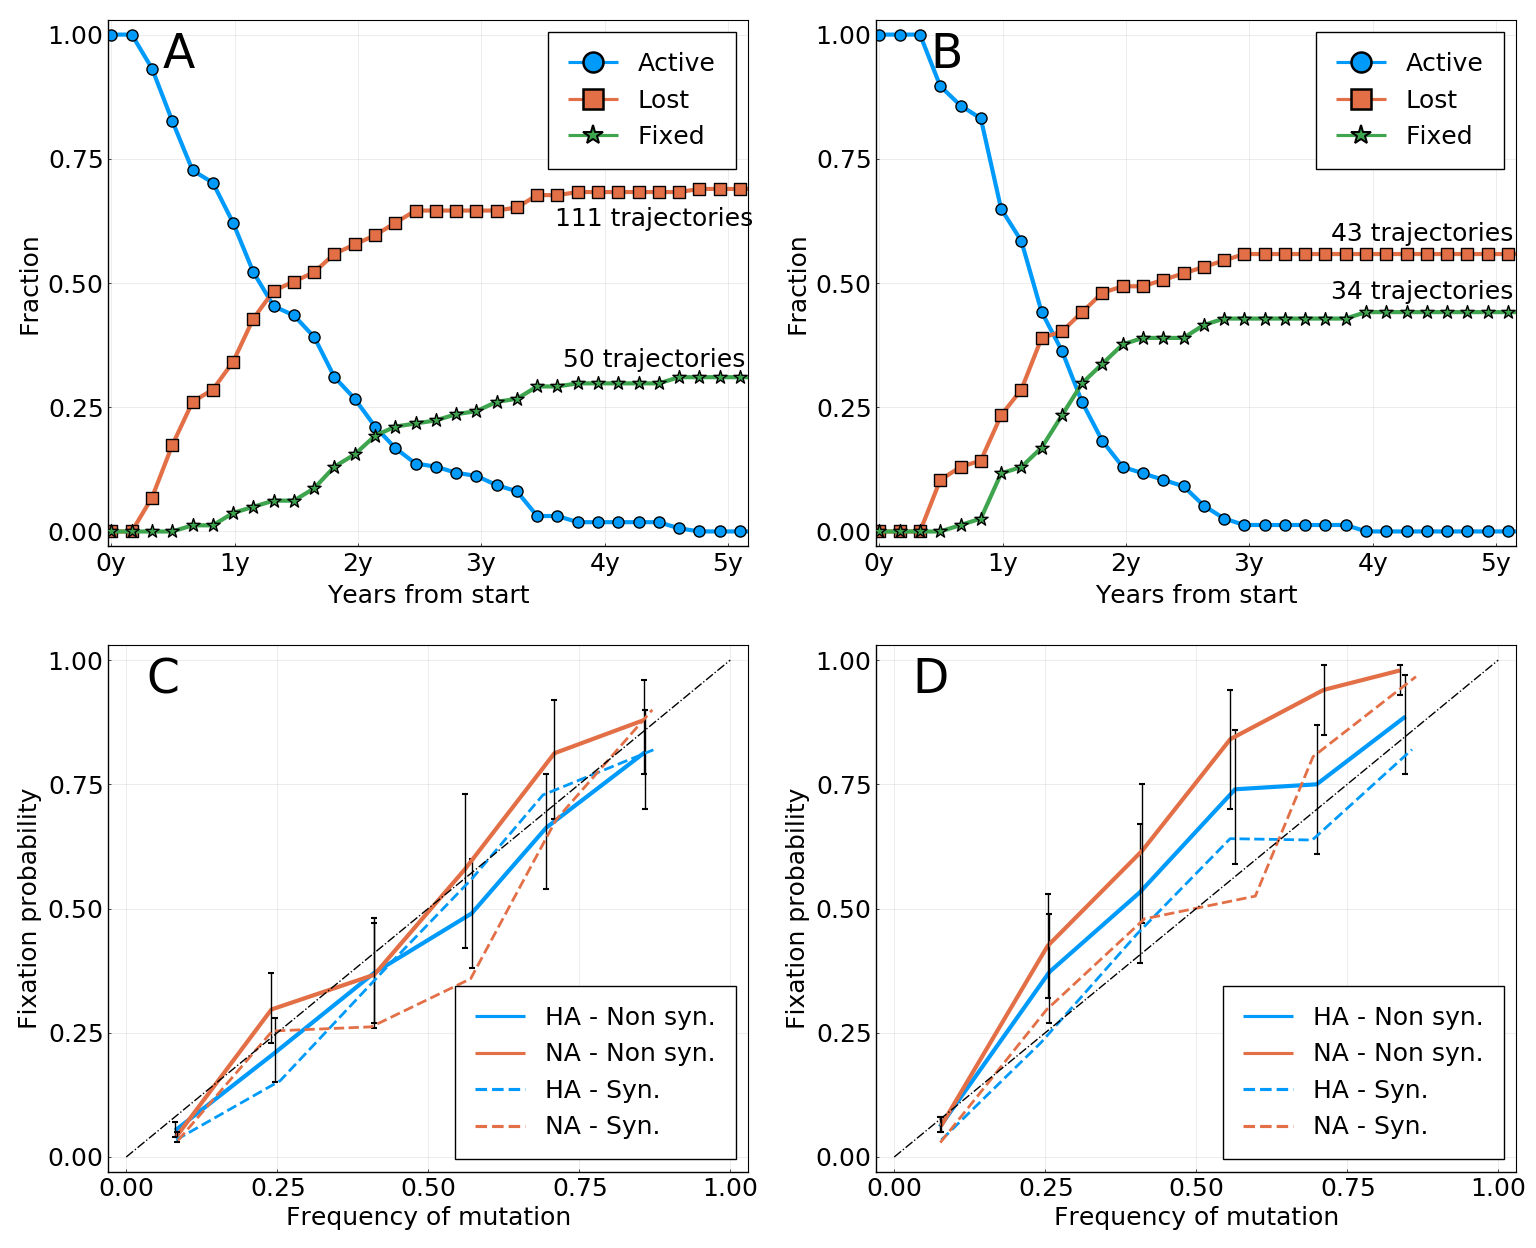
\includegraphics[width=0.9\textwidth]{./Figures/Panel2.png}
		\caption{\textbf{A}: Sketch of the idea behind the short term prediction of frequency trajectories. Given a mutation that we have seen increasing in frequency and that we "catch" at frequency $f_0$ at time $t_0$, what can we say about the distribution of future frequencies $P_{\Delta t}(f)$? \textbf{B}: All frequency trajectories of amino acid mutations in the HA gene that were absent in the past, are seen around 30\% frequency at time $t_0=0$, and are based on more than 10 sequences at each time point. Red curves represent mutations that will ultimately fix, blue the ones that will be lost, and black the ones for which we do not know the final status. Dashed horizontal lines (blue and red) represent loss and fixation thresholds. \textbf{C}: Distribution of future frequencies $P_{\Delta t}(f)$ for the trajectories shown in panel \textbf{B} and for specific values of $\Delta t$. The data is shown by the circles, the lines are a smooth fit to the distribution and should be seen as a guide for the eye. }
		\label{fig:panel2}
	\end{figure}

	\subsection*{Long term prediction}

	The future values of a frequency trajectory $f(t)$ do not seem to be easily predictable. However, another way to predict evolution is to focus not on dynamical details of the frequency of a mutation but rather on the probability that a mutation fixes in the population. For influenza, this question is of particular importance as the knowledge of the future H3N2 population and of the mutations it acquired is critical to the development of a vaccine. Here, we use the past frequency trajectories to assess our ability to predict fixation of mutations in the population. Since most mutations define a unique clade in the phylogenetic tree of HA or NA genes, this amounts to predicting which clade will be the ancestor of the future influenza population. \\
	We first estimate the number of frequency trajectories that either fix in the population or are lost, as well as the time it takes for one or the other to happen. For this, we consider the 106 new amino acid mutations in HA that are seen at least once above a frequency of 25\%. Panel \textbf{A} of figure~\ref{fig:panel3} shows the fraction of frequency trajectories corresponding to these mutations that either fix, are lost or remain active as a function of the time elapsed since they were first seen above 25\% frequency. It is clear from this plot that most mutations are either lost or become fixed in a few years, with no trajectory remaining active after 6 years. It is relevant to note that this value of 6 years is also the typical coalescence time observed in phylogenetic trees of H3N2 influenza. We also note that the fraction of lost trajectories increases sharply at small times, indicating that many mutations observed at a significant frequency are lost relatively quickly, while it takes longer to fix a mutation in the whole population. \\

	\begin{figure}
		\centering
		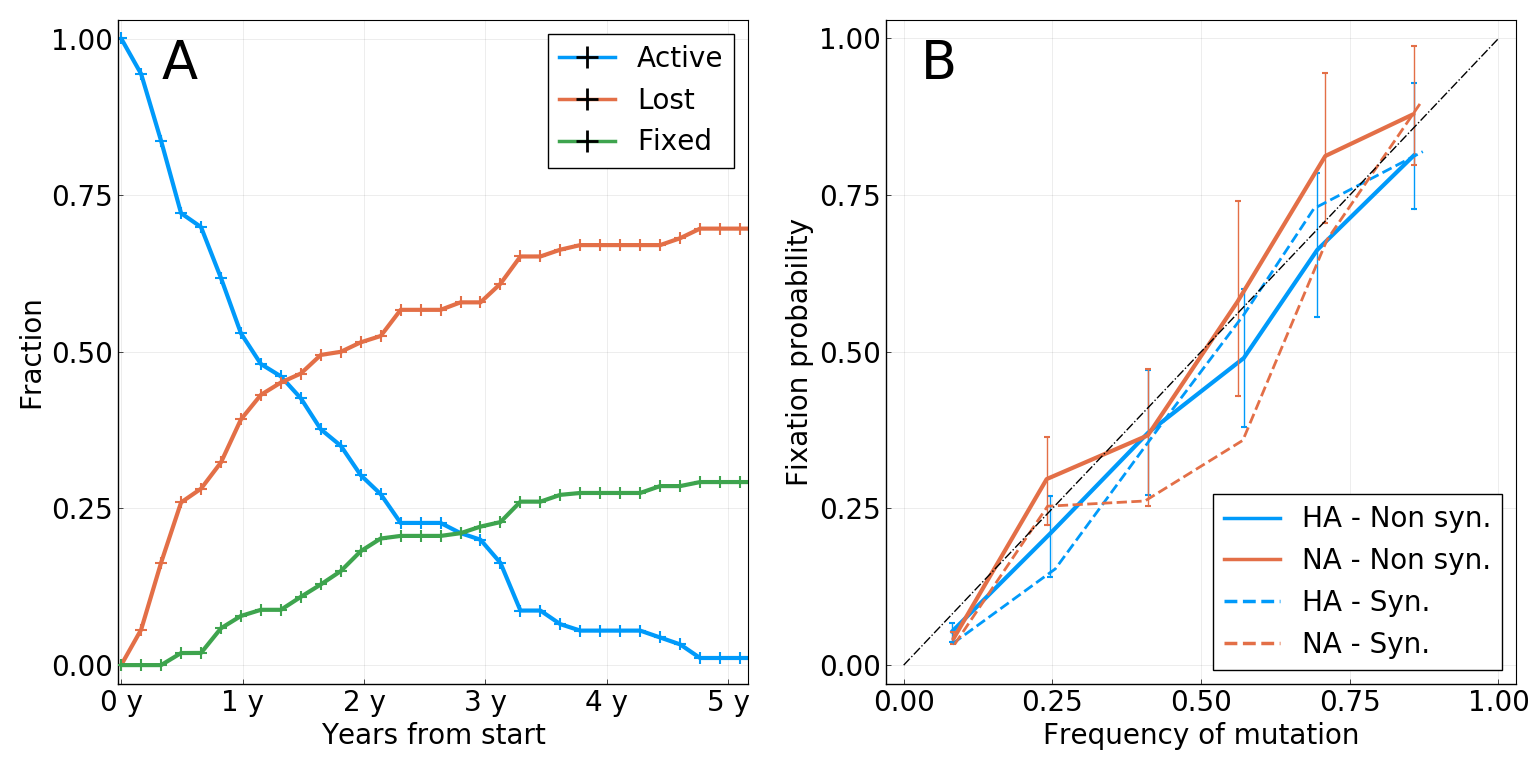
\includegraphics[width=0.9\textwidth]{./Figures/Panel3.png}
		\caption{\textbf{A}: Activity of all rising frequency trajectories seen above 25\% frequency. \textbf{B}: Probability of fixation of a mutation (amino acid or synonymous) $P_{fix}(f)$ as a function of the frequency $f$ at which it is measured. Only new mutations are considered, \emph{i.e.} mutations that were absent in the past. The diagonal dashed line is the expectation from a neutrally evolving population.}
		\label{fig:panel3}
	\end{figure}

	We then examine the probability of mutations to fix in the population as a function of the frequency at which they are seen. For different values of frequency $f$, we consider all trajectories that started at a null frequency and are seen in the interval $[f - 5\%, f + 5\%]$ at any given time. The probability of a mutation fixing given that it is seen at frequency $f$, $P_{fix}(f)$, is then estimated by the fraction of those trajectories which terminate at a frequency larger than $95\%$, \emph{i.e.} our fixation threshold. \\
	Results are shown for proteins HA and NA in the panel \textbf{B} of figure~\ref{fig:panel3} by plotting $P_{fix}(f)$ as a function of $f$. We notice that for both these proteins, the probability of fixation of a new mutation seen at frequency $f$ is very close to $f$ itself, that is $P_{fix}(f)\simeq f$. This result is quite surprising, as this is exactly what is expected from a population evolving in the \emph{absence} of selection. Indeed, in a neutrally evolving and structure-less population of constant size $N$ such as in the Wright-Fisher model~\cite{10.1080/10635150500354860}, the probability that any individual ultimately becomes the ancestor of all the future population is $1/N$. A mutation or trait appearing at frequency $f$ is shared by $f\cdot N$ individuals, and the probability for one of them to become the ancestor of all the future population is $f\cdot N/N=f$. Thus, the probability of this mutation or trait to fix in the population is equal to its current frequency, a case which we will refer to as the neutral expectation. Panel \textbf{B} of figure~\ref{fig:panel3} indicates that mutations in the surface proteins of H3N2 influenza are in good agreement with the neutral expectation.\\
	This is surprising, since influenza is usually described as being under strong selective pressure to evade its host's immune systems. If strong selection was present, we would expect rising amino acid mutations to fix at a higher frequency than the one at which they are measured. In an extreme case where most trajectories would be clean sweeps, $P_{fix}(f)$ should be close to $1$ for all but very small values of $f$. \\
	To investigate further, we try to find groups of mutations that deviate from the neutral expectation of figure~\ref{fig:panel3}. We first turn to the \emph{Local Branching Index} (LBI), a quantity calculated for each node in a phylogenetic tree that indicates how dense the branching of the tree is around that node. LBI has previously been successfully used as a predictor of the future population of influenza~\cite{neher_predicting_2014}, and is arguably a good proxy for the fitness of a leaf (\emph{i.e.} a strain) or an ancestral node in a tree. Here, we define the LBI of a mutation at date $t$ as the average LBI of strains that carry this mutation and that were sampled in the time bin corresponding to $t$. This effectively represents the average density of the tree around nodes that carry the mutation. We then reproduce the plot of figure~\ref{fig:panel3}, but this time dividing trajectories into two groups: those corresponding to mutations with higher LBI, meaning that their LBI is higher than the median value recorded for mutations present in the same frequency bin, and those with lower LBI. Panel \textbf{A} of figure~\ref{fig:panel4} shows this plot for HA. Because both groups are again consistent with neutral evolution, we see that LBI carries very little information on the probability of fixation of a mutation as both subgroups are again similar to the neutral expectation. \\
	Next, we concentrate on previously reported antigenic sites in the HA protein, referred to as \emph{epitope} positions. These sites are considered responsible for the ability of H3N2 to evade immune systems, and mutations at these locations should therefore be under strong selection. Four lists of relevant epitope positions from different authors are used, comprising from 7 to 129 positions in the sequence of the HA1 protein~\cite{Koel976, luksza_predictive_2014, Shih6283, wolf_long_2006}. Panel \textbf{B} of figure ~\ref{fig:panel4} shows the $P_{fix}(f)$ as a function of $f$ curve for the four lists of epitopes. Results show that mutations on epitope sites as reported in~\cite{Koel976, luksza_predictive_2014} have slightly higher chances of fixation, while no clear difference is found in the case of~\cite{Shih6283, wolf_long_2006}. However, even in the former case, observations are different from what one would expect if the dynamics where dominated by selective sweeps. Several other ways of looking at subset of mutations or positions reach the same result: fixation probability hardly deviates from the neutral expectation (see figure \ref{fig:pfix_v_freq_misc} in SM). [I should maybe add something saying that those epitope positions might have been found \emph{using} the fact that sweeps often take place there? Is that the case? depends on authors most likely. EDIT: Wolf et al. seems to report all sites that are somehow important to the immune system. The others have a selection of those. For Koel and Luksza, it seems to be based on the fact there have been sweeps at these positions (in an indirect manner). Should read papers more carefully. Also, Koel et al. has 7 epitope positions, so error bars on the $y$-axis must be huge. And finally: taking RBS positions actually increases $P_{fix}(f)$ significantly (Koel et al. takes positions close to the RBS).]\\
	\pierre{Write something on panels \textbf{C} and \textbf{D}, \emph{i.e.} binary mutations and mutations found once or more in the tree.}

	Motivated by the fact that the number of influenza cases varies strongly with the seasons in non-tropical regions, we turn to ways of classifying mutations that are not based on genomes and phylogeny but rather on "epidemiological" observations. First, a score reflecting \emph{geographical spread} is assigned to each mutation. It is based on the entropy the regional distribution of each mutation (details in Methods). We also use the age of trajectories as a second score, that is, for each frequency $f$, the amount of time between the date at which the corresponding mutation is first seen, and the date at which it reaches frequency $f$. \\
	Fixation probabilities as a function of observed frequency with mutations classified by higher or lower values of these scores (\emph{i.e.} higher or lower than the median of observed values) are shown in panels \textbf{A} and \textbf{B} of supplementary figure~\ref{fig:geospread_and_time}. These two scores also allow a quantitatively moderate distinction between mutations: for a given frequency $f$, mutations found in many regions or that are older (in the sense that they have taken more time to reach frequency $f$) tend to fix more often than geographically localized mutations or more recent ones. These two scores are in fact correlated, with older trajectories representing mutations that are more geographically spread, as can be seen in figure~\ref{fig:geospread_v_time} of SM. \\
	A natural way to explain these observations would be to refer to the seasonal characteristics of H3N2. In temperate regions, the number of H3N2 infections drastically increases during winter, leading to an at first rapidly growing and then declining population of viruses. For this reason, one could imagine that some mutations rise in frequency in an "opportunistic" way during an epidemic season, but do not survive the following decline in population size. For the same reason, mutations that are localized in a particular region might mostly be due to the epidemic season specific to that region. \\
	However, it is important to note that verifying this kind of hypothesis remains challenging with the available data. Indeed, supplementary figures~\ref{fig:nseq_per_year} and ~\ref{fig:nseq_per_month} clearly shows that sequence are not uniformly sampled in either in time or space: some countries or regions sequence much more than others, but also do so at a varying intensity in time (see for instance Oceania samples in figure~\ref{fig:nseq_per_year}). Frequency of mutations might thus be amplified through different sampling biases, making the connection between geographic spread, seasonality and mutation frequency non trivial to measure. It is however interesting to observe that quantities based on the population's geographical and temporal structure can apparently give as much or more information on fixation probability and predictability than genomic or phylogenetic ones. 

	\begin{figure}
		\centering
		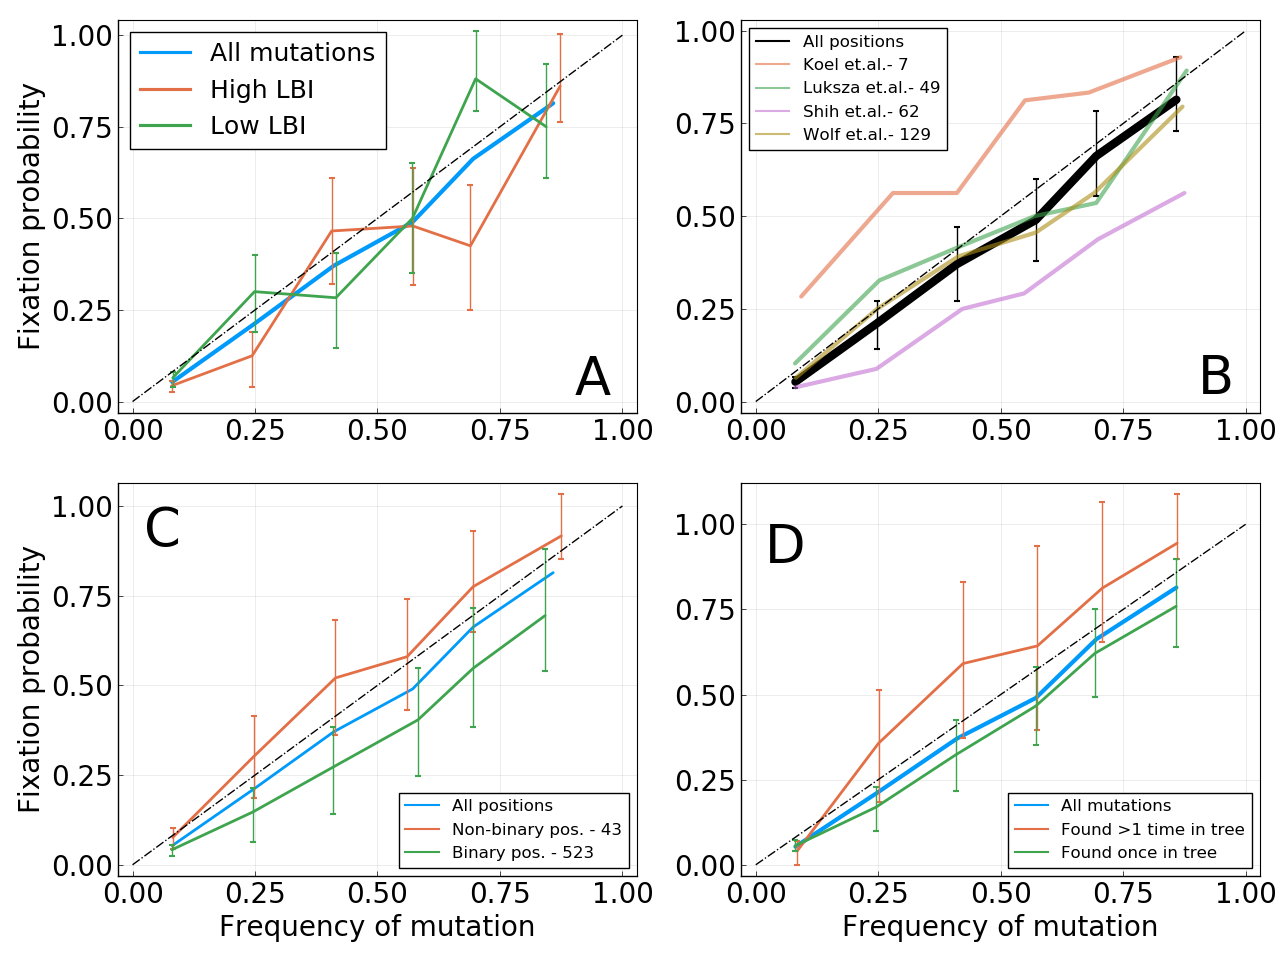
\includegraphics[width=0.9\textwidth]{./Figures/Panel4.png}
		\caption{Fixation probability $P_{fix}(f)$ as a function of frequency. \textbf{A}: Mutation with higher or lower LBI values, based on their position with respect to the median LBI value. \textbf{B}: Different lists of epitope positions in the HA protein. The authors and the number of positions is indicated in the legend. \textbf{C}: Mutations for binary positions, \emph{i.e.} positions for which we never see more than two amino acids in the same time bin. \textbf{D}: Mutations that appear once or more than once in the tree for a given time bin.}
		\label{fig:panel4}
	\end{figure}

	\subsection*{A simple model}
	\label{sub:a_simple_model}

	Quick summary. The results shown in figures~\ref{fig:panel3} and \ref{fig:panel4} are surprising. One could argue that the apparently neutral behaviour of mutations is due to strong genetic linkage inside each protein and high competition between different adaptive mutations. We design a simple model of population evolution based on the \texttt{ffpopsim} simulation software to test this hypothesis~\cite{10.1093/bioinformatics/bts633}. The model represents a population of binary genomes of length $L=200$ evolving in a fitness landscape that changes through time. 
	Two different fitness landscapes are used, described below. \\
	First, we use an additive fitness function, with sequence $(x_1\ldots x_L)$ having a fitness $h_1 x_1 + \ldots + h_L x_L$. This implies that for a given genome position $i$, the trait $x_i = 1$ is favored if $h_i>0$ whereas  $x_i = -1$ is favored if $h_i<0$. All $h_i$'s have the same amplitude, and only their signs matter. Every $\Delta t$ generations, we randomly choose a position $i$ and flip the sign of $h_i$, effectively changing the fitness landscape. Individuals in the population now have the opportunity to make an adaptive mutation at site $i$ giving them a fitness advantage $2\vert h \vert$. However, because of the absence of recombination, a genome that has adaptively mutated at $i$ might also carry non-optimal mutations referred to as mutational load. Each "flip" in the fitness landscape will thus create a competition between genomes carrying the adaptive mutation as well as their own mutational load. \\
	To increase competition between genomes, we design a second model that includes epistasis. Once again, the baseline fitness of a genome is an additive function, this time with values of $h_i$ that do not change through time. Every $\Delta t$ generation, we now introduce "antibodies" that target a specific sub-sequence of length $l=5$, noted $(x^{ab}_{i_1}, \ldots, x^{ab}_{i_l})$. The positions $(i_1\ldots i_l)$ are chosen at random, while the value $x^{ab}_i$ is chosen to be the dominant trait at position $i$. Genomes that include the \emph{exact} sub-sequence targeted by the antibody suffer a strong fitness penalty. However, a single mutation away from that sub-sequence removes this penalty, resulting in a fitness landscape with very strong epistasis. This has the effect of triggering a strong competition between adaptive mutations: for a given antibody, $l=5$ possible mutations are now adaptive, but combinations of these mutations do not bring any fitness advantage. \\
	Having simulated populations in these two fitness landscapes, we perform the same analysis of frequency trajectories as for the real influenza data. Figure~\ref{fig:simulations} of the SM shows the $P_{fix}(f)$ as a function of $f$ curve for the two models and for different values of the inverse rate of change $\Delta t$ of the fitness landscape. For all models, this curve deviates significantly from the diagonal. This is most evident in the case without antibodies and with a very long rhythm of change $\Delta t=1000$. In this scenario, rising mutations almost always fix in the population, with $P_{fix}(f)\simeq 1$ for any $f$ larger than a few percent. This is corroborated by visual inspection of the trajectories, which shows that evolution in this regime is driven by regular selective sweeps that take a typical time of $\sim 400$ generations. In other regimes, with smaller $\Delta t$ or with the introduction of antibodies, $P_{fix}(f)$ typically becomes smaller and closer to the diagonal. However, even in an extremely fast changing fitness landscape with $\Delta t=10$, that is about 40 changes to the fitness landscape in the time it would take a selective sweep to go from 0\% to fixation, $P_{fix}(f)$ still significantly differs from $f$. \\
	These models do not claim to be in any way realistic, and even less to be a good representation of the evolution of influenza or viruses. What we learn from them and from figure~\ref{fig:simulations} is that it is not a trivial task to design a model which includes selection and yet has a behaviour that is in apparent good agreement with a neutral evolution scenario, such as what figure~\ref{fig:panel3} shows. This makes the results of the previous section all the more interesting, as influenza is generally regarded as being under strong selection in a changing fitness landscape. In other words, the results of figure~\ref{fig:panel3} may not be be regarded as obvious manifestations of genetic linkage and clonal interference. 

	\subsection*{Why do predictions work}

	Results that we obtained on the frequency trajectories of mutations are in good agreement with what is expected of a neutrally evolving population. What is even more surprising is that the Local Branching Index, a quantity that has previously been thought of as a good approximation for the fitness of strains, does not seem to contain any information on whether a specific mutation is going to fix or not, see figure~\ref{fig:panel4}. However, LBI has also been demonstrated to be a good predictor of the  future influenza population. This raises an obvious question: why does predicting the evolution of influenza work at all? \\
	We investigate this using a subsample of the HA sequences used in the previous sections. We decide to work with larger non-overlapping time bins of 4 months. For each such time bin from year 2003 to 2019, we randomly sample 100 HA sequences, reaching a total of 4402 (some 4 month intervals contain less than 100 sequences in total). A tree is also inferred using those sequences, and the LBI of each node in that tree is computed.\\
	Each time bin is considered as a snapshot of the H3N2 influenza population for a given date. Predicting the evolution of the influenza population consists of obtaining as much information as possible on the sequences contained in a future time bin $t+\Delta t$, using only sequences in time bin $t$ and before. Sequences in $t$ are referred to as the \emph{present} population, and sequences in $t+\Delta t$ as the future population. We attempt to measure the efficiency of two predictors consisting of a single sequence: the sequence of the strain with the highest LBI, and the amino acid consensus sequence of members of the present population (see Methods for a definition of the consensus sequence). The choice of the consensus sequence as a predictor is motivated by the fact that it can be shown to be the best possible long term predictor for a neutrally evolving population if Hamming distance is used as a measure (see SM). However, it is important to note that this sequence does \emph{not} necessarily exist in the population. Our procedure is then the following: for a given 4 month time bin $t$, that is for a given "present" population, we compute the \emph{average Hamming distance} between the sequence of the predictor strain and the sequences of future populations at times $t+\Delta t$, for $\Delta t$ comprised between $0$ and $32$ months. Results are then averaged over all  possible values of $t$, giving us an average efficiency of a predictor over 16 years of influenza evolution. \\
	The top panel in figure~\ref{fig:panel5} shows the results of this procedure, also comparing them to a predictor based on a randomly chosen strain. It is very clear that both predictors, the LBI-based one and the consensus, are consistently and significantly more accurate than a random pick in the present population. This can be taken as both a positive sign and a confirmation of previous results: it is to some extent possible to predict the evolution of influenza in the sense that one can do better than a purely random guess. However, what is striking is the high similarity between the predictions of the top-LBI strain and the consensus sequence. Moreover, the consensus sequence fares slightly but consistently better than the LBI, even if only slightly. This is surprising in that the consensus sequence is the best possible long-term possible predictor for a neutrally evolving population, whereas the LBI was designed as an approximate measure of fitness of strains. \\
	An explanation for this observation is that the LBI tends to be high for nodes in a tree that are close to the root of a dense and large clade. If we think of the influenza population as divided into a few different clades, and if the strains with the maximal LBI are close to the root of the largest of those clades, then it may also be that their sequence is close to the consensus of the whole population. To test that hypothesis, we measure the hamming distance from the sequence of the top LBI strain to the consensus sequence for populations of all time bins. Panel \textbf{B} of figure~\ref{fig:panel5} shows these distances, scaled with respect to an average strain (details in caption). It clearly shows that the top-LBI strain and the consensus sequence are indeed quite similar: out of 48 time bins, only once is the sequence of the top-LBI strain farther away from the consensus than the average sequence is. Moreover, the sequence of the top-LBI strain \emph{exactly} matches the consensus in 23 cases. \\


	\begin{figure}
		\centering
		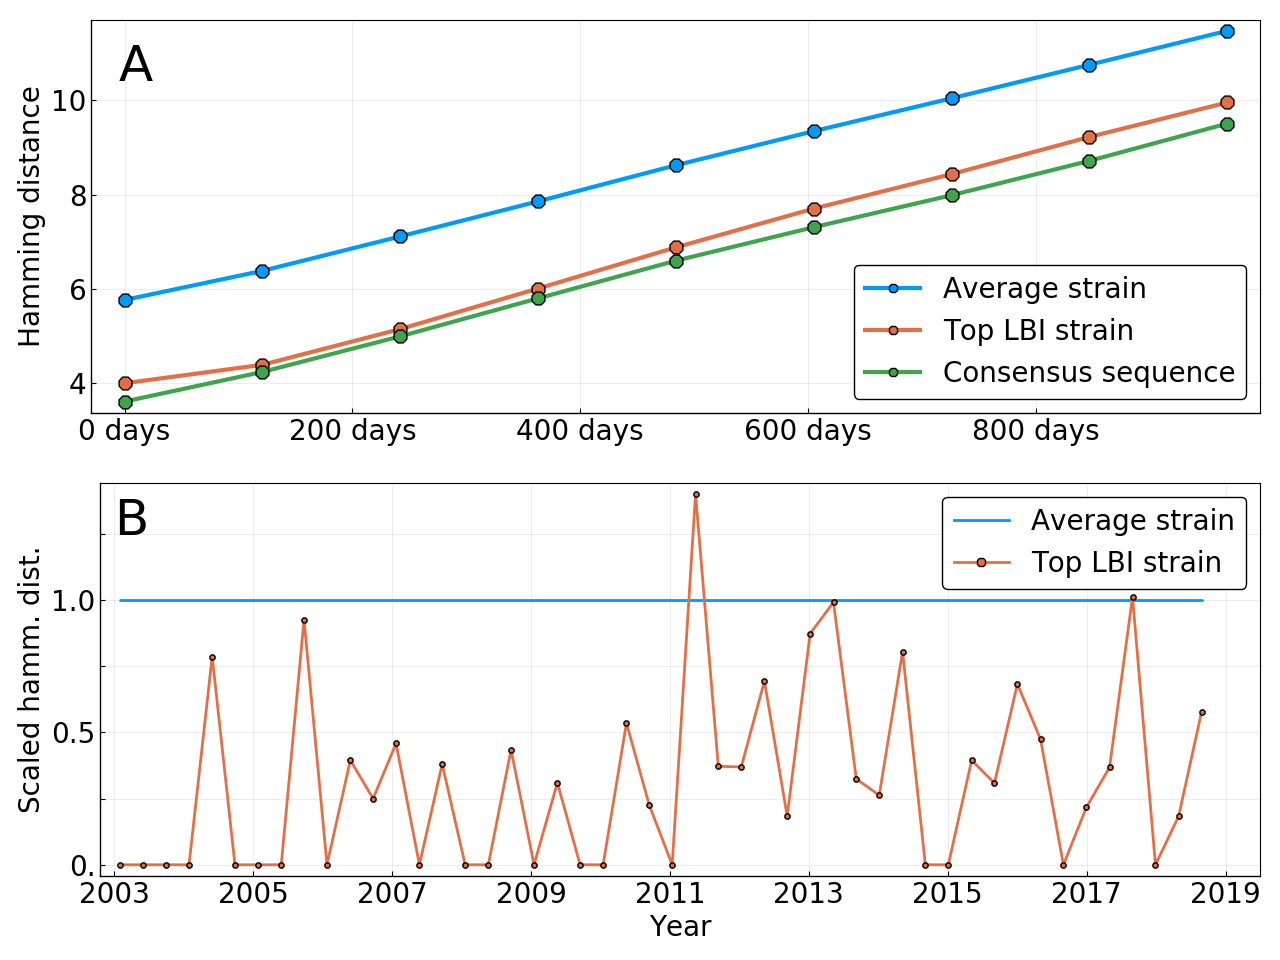
\includegraphics[width=0.9\textwidth]{./Figures/Panel5.png}
		\caption{\textbf{A}: Average Hamming distance of the sequences of different predictors to HA sequences of future influenza populations, themselves averaged over all "present" populations from year 2003 to 2019. Predictors are: a randomly picked sequence in the present population; the sequence of the strain with the highest LBI in the present population; the consensus sequence of the present population. \textbf{B}: Scaled Hamming distance between the sequence of the top LBI strain and the consensus sequence for populations at different dates. The scaling is such that for each date, the Hamming distance between a strain from the population and the consensus is on average $1$. The strain with the highest LBI is almost always closer to the consensus sequence than the average strain.}
		\label{fig:panel5}
	\end{figure}

% section results (end)

\section*{Discussion} % (fold)
\label{sec:discussion}

The idea of predicting the outcome of a mutation is based on two assumptions: significant fitness effects between genomes carrying different mutations and a stable enough environment. These two conditions are essential for the existence of a consistent selective pressure on mutations, which is expected to give inertia to frequency trajectories of mutations, thus making them predictible. We simulated a population having such a selective pressure in  section \ref{sec:a_simple_model} and found indeed that as long as the fitness landscape does not change too rapidly (\emph{i.e.} small $dt$ limit), frequency trajectories are predictible to some extent. \\
Methods for predicting the future evolution of influenza usually rely on modeling how this selection operates and on finding the values of fitness for strains or mutations. In this work, we tries to understand whether the selective pressure acting on influenza is strong and consistent enough to make frequency trajectories of mutations follow "inertial" patterns such as selective sweeps. By analyzing 19 years of evolution of the HA and NA genes in h3n2 influenza, we find that these trajectories do not behave in an easily predictible way. On the short time scale, not much can be said about the future frequency values or even the direction of a rising trajectory. On the longer time scale, we find that the probability of an amino acid mutation to fix is in very good agreement with what is expected of a neutrally evolving population. \\
Usual prediction tools add surprisingly little information to this. On the one hand, Mutations at some epitope positions are slightly more likely to fix than ones at other positions, but their probabilty of fixation remains very close to the neutral expectation. On the other, the Local Branching Index seems to carry no information at all on probability of fixation. It is interesting to note that other simple quantities also give an indication on probability of fixation, such as the number of times the mutation appears in the tree, the restriction to positions that never see three amino acids compete at the same time, or the age and geographical spread of the mutation (SM figure \ref{fig:geospread_and_time} for the latter). \\
These results naturally trigger the question of the reasons why prediction methods have been found to work. We focused on the surprising case of LBI. In the last section, we showed that the strain with the highest LBI in a given present population is a better predictor of the future population than a randomly picked one. However, we also find that the very simple method of taking the consensus sequence of all present strains performs slightly but consistently better than the LBI. Interestingly, the consensus sequence is the best possible predictor for a neutrally evolving population, and does not model fitness in any way. Thus, even though the LBI claims to approximate the fitness of strains based on their genealogy, it may be a good predictor for different reasons. \\
Overall, these results indicate that the potential predictibilty of the evolution of influenza is fairly low, challenging the views that this evolution operates under a strong and consistent selective pressure. On the contrary, we fail to find evident signs of a such a selective pressure and show that the LBI, designed to measure fitness, may not work for the "right" reasons. 


Quick list of what should be said: 
\begin{itemize}
	\item Flu is usually seen as evolving under strong selection. Predicting its evolution should thus rely on finding how this selection operates, and finding which strains are the most fit according to it. 
	\item Analysing 19 years of flu evolution, we find that frequency trajectories of mutations in the HA and NA proteins do not behave in an obviously predictable way. More precisely, the "inertia" or "persistence time" of these trajectories is at best quite short, and seeing a mutation rising in frequency does not tell us much on its future. 
	\item We also find that the probability of a specific mutation to fix in the flu population is in very good agreement from what is expected of a neutrally evolving population. Usual predictive tools such as the LBI or the epitope positions on the HA protein do not add much information to the probability of fixation. However, we find evidence that population geographical and temporal structure does give a limited amount of information. 
	\item Using a simulation of a constant size population evolving under selection, we demonstrate that the previous findings are not easily reproduced by usual views of population dynamics. Simple but reasonable models do not behave in an apparently neutral manner
	\item Surprised by these observations, we wonder whether predictive tools such as the LBI work at all. By using hamming distance to future populations as a measure, we show that the strain with the highest LBI is indeed a good prediction of future sequences in the sense that it is better than a random pick. However, we also find that the consensus sequence fares consistently better than the LBI. This is in perfect agreement with previous results, since the consensus sequence is the best possible predictor for a neutrally evolving population. 
	\item Overall, this work leaves us with more questions than we started with. It shows that the usual views of evolution of influenza may be quite inaccurate and potentially misleading. Indeed, selection may be too small to be easily detected by the methods we used here, or operates in a way that we do not understand. It also suggests that population structure (geographical and temporal) should not be discarded as it may play an important role in this evolution. 
\end{itemize}

% section discussion (end)

\section*{Methods} % (fold)
\label{sec:methods}

\subsection*{Data} % (fold)
\label{sub:data}

% subsection data (end)

\subsection*{Frequency trajectories} % (fold)
\label{sub:frequency_trajectories}
	
	For a set of sequences in a given time bin, we compute frequencies of amino acids at each position by simple counting. We make the choice of not applying any smoothing method in an attempt to be as close to the data and "model-less" as possible. This is especially important for the short term prediction of frequency trajectories, as estimations of the "persistence time" of a trajectory might be biased by a smoothing method. \\
	We compute frequency trajectories based on the frequencies of amino acids. A trajectory begins at time $t$ if an amino acid is seen under the lower frequency threshold of 5\% (resp. above the higher threshold of 95\%) for the two time bins preceding $t$, and above this lower threshold (resp. below the higher threshold) for time bin $t$. It ends in the reciprocal situation, that is when the frequency is measured below the lower threshold (resp. above the higher threshold) for two time bins in a row. \\
	In order to avoid estimates of frequencies that are too noisy, we only keep trajectories that are based on a population of at least 10 sequences for \emph{each} time bin. As said in the Results section, we also restrict the analysis to trajectories that begin at a $0.$ frequency, in part to avoid double counting. We find a total of 460 such trajectories. However, only 106 reach a frequency of 20\%, on which figure~\ref{fig:panel3} is based for instance.  

% subsection frequency_trajectories (end)

\subsection*{Local Branching Index} % (fold)
\label{sub:local_branching_index}
		
	LBI was introduced in \cite{neher_predicting_2014} as an approximation of fitness in populations evolving under persistent selective pressure that is fully based on a phylogenetic tree. It relies on the intuition that the tree below high-fitness individuals will show dense branching events, whereas absence of branching is a sign of low-fitness individuals. Quantitatively, the LBI $\lambda_i(\tau)$ of a node $i$ is the integral of all of the tree's branch length around $i$, with an exponentially decreasing weight $e^{-t/\tau}$ with $t$ being the branch length. $\tau$ is the time scale for which the tree is informative of the fitness of a particular node. Here, we use a value of $\tau$ equal to $T_C\simeq6$ years, the coalescence time for influenza H3N2 strains, converted to units of tree branch length through the average nucleotide substitution rate ($\simeq 4\cdot 10^{-3}$ substitutions per site per year for HA). We have observed that given our method to predict the future from present populations corresponding to time bins of 4 months, changing the value of $\tau$ has little effect on the pick of the top LBI strain. By retrospectively optimizing its value, it is possible to reduce the average distance to the population 2 years ahead by $\sim0.25$ amino acids on average, making the LBI method almost as good as the consensus on figure~\ref{fig:panel5}. 

% subsection local_branching_index (end)

\subsection*{Measuring the geographical spread of a mutation} % (fold)
\label{sub:measuring_the_geographical_spread_of_a_mutation}
	For a mutation $X$ we define its regional distribution using the numbers $n_r(X)$ that represent the number of sequences sampled in region $r$ that carry $X$. Regional weights are then defined as 
	$$ w_r(X) = \frac{n_r(X)}{\sum_{r}n_r(X)}.$$
	We can then measure the geographical spread $G(X)$ of $X$ by using the Shannon entropy of the probability distribution $w_r(X)$: 
	$$G(X) = \sum_r w_r(X)\log(w_r(X)).$$
	$G(X)$ is a positive quantity that is larger when $X$ is equally present in many regions, and equal to zero when $X$ is concentrated in only one region.\\
	Region used are the ones defined in the \texttt{nextstrain} tool~\cite{10.1093/bioinformatics/bty407}. Those are {North America}, {South America}, {Europe}, {China}, {Oceania}, {Southeast Asia}, {Japan \& Korea}, {South Asia}, {West Asia}, and {Africa}.
% subsection measuring_the_geographical_spread_of_a_mutation (end)

\subsection*{Consensus sequence} % (fold)
\label{sub:consensus_sequence}
	Given a set of $N$ sequences $(\sigma^1,\ldots,\sigma^N)$ based on an alphabet $\mathcal{A}$ (\emph{e.g.} $\mathcal{A}$ has 20 elements for amino acids, 4 for nucleotides), we can define a \emph{profile} distribution $p_i(a)$ by the following expression:
	$$ p_i(a) = \sum_{n=1}^N \delta_{\sigma^n_i,a} $$ 
	where $i$ is a position in the sequence, $\sigma^n_i$ the character appearing at position $i$ in sequence $\sigma^n$, $a$ a character of the alphabet and $\delta$ the Kronecker delta. The profile $p_i(a)$ simply represents the fraction of sequences which have character $a$ at position $i$. \\
	We then simply define the consensus sequence $\sigma^{cons}$ such that 
	$$\sigma^{cons}_i = \text{argmax}_a \;p_i(a).$$
	In other words, the consensus sequence is the one that has the dominant character of the initial set of sequences at each position.   
% subsection consensus_sequence (end)

\subsection*{Earth Mover's Distance} % (fold)
\label{sub:earth_mover_s_distance}

	In order to measure the distance of several predictor sequences to the future population, we rely on the \emph{EarthMover's Distance} (EMD), a metric commonly applied in machinelearning to compare collections of pixels or words \cite{710701,10.5555/3045118.3045221}. Here, we apply it to compute the distance between the sequences of two populations, noted as $\mathcal{X} = \left\{(x^n, p^n)\right\}$ and $\mathcal{Y}=\left\{(y^m,q^m)\right\}$ with $n\in\{1\ldots N\}$ and $m\in\{1\ldots M\}$. In this notation, $x^n$ and $y^m$ are sequences, and $p^n$ and $q^m$ are the frequencies at which these sequences are found in their respective populations. For convenience, we also define $d_{mn} = H(x^n,y^m)$ as the Hamming distance between pairs of sequences in the two populations. \\
	We now introduce the following functional
	$$ F(\mathbf{w}) = \sum_{n,m} d_{nm}w_{nm}, $$
	with $\mathbf{w} = \{w_{nm}\}$ being a matrix of positive weights. The EMD between the two populations $\mathcal{X}$ and $\mathcal{Y}$ is now defined as the minimum value of function $F$ under the conditions 
	\begin{equation*}
		% \begin{split}
			\sum_{n=1}^N w_{nm} = q^m,\;\; \sum_{m=1}^M w_{nm} = p^n, \,\text{and}\;\; w_{nm}\geq 0
		% \end{split}
	\end{equation*}
	Intuitively, the weight $w_{nm}$ tells us how much of sequence $x^n$ is "moved" to sequence $y^m$. The functional $F$ sums all of these moves and attributes them a cost equal to the Hamming distance $d_{nm}$. The conditions on weights in $\mathbf{w}$ ensure that all the weight $p^n$ of $x^n$ is "moved" to elements in $\mathcal{Y}$ and vice versa. \\
	The minimization is easily performed by standard linear optimization libraries. Here, we use the Julia library {JuMP}~\cite{DunningHuchetteLubin2017}.
% subsection earth_mover_s_distance (end)

% section methods (end)

\bibliographystyle{unsrt}
\bibliography{references}

\newpage 

\section*{Supplementary material} % (fold)
\label{sec:supplementary_material}

\subsection{Consensus sequence as a predictor for neutrally evolving populations} % (fold)
\label{sub:consensus_sequence_as_a_predictor}
	
	We consider the case of a neutrally evolving and structure-less population, such as the one in the Wright-Fisher model of evolution~\cite{10.1080/10635150500354860}. At an initial time $t=0$, the population consists of $N$ individuals with genomes $(\sigma^1\ldots\sigma^N)$ of length $L$ (not necessarily distinct). \\
	% We introduce the distribution $f(\sigma)$ representing the frequency at which a particular genome $\sigma$ appears in the population, that is 
	% $$ f(\sigma) = \frac{1}{N}\sum_{n=1}^N \delta_{\sigma, \sigma^n}$$
	% where $\delta_{x,y}$ is the Kronecker delta. \\
	We make two hypotheses about this population. We first suppose that \emph{no} mutations occur during the evolution of this population. This may seem surprising and is of course not true in the case of influenza. This assumption is however in line with the fact that the object of this work is to predict the outcome of \emph{already existing} mutations in the influenza population. The prediction of mutations that we have not yet seen is not in its scope. Thus, assuming that no new mutations take place can be seen as a simple way to model the fact that we have no information about such events. \\
	The second assumption is that the population evolves in a completely neutral way, meaning that the average number of descendants of each genome $\sigma^n$ is the same. Let us now consider the population after it has evolved for a long time $t\gg T$ where $T$ is the typical coalescence time (for the Wright-Fisher model, $T=2N$). At this point, all individuals in the future population will descend from a unique individual $n_0$ in the $t=0$ population. Our two hypotheses now allow us to make two statements. First, since no new mutations are allowed, the population at $t\gg T$ will be clonal, with all individuals having genome $\sigma^{n_0}$. Second, since the evolution is neutral and does not favour any genome in particular, the probability that $\sigma^{n_0}$ is equal to a given genome $\sigma$ is $1/N$. In other words, the probability that a genome at $t=0$ ultimately becomes the ancestor of all the future population is equal to its frequency in the $t=0$ population. \\

	We now try to find the genome $\sigma$ that best predicts the future population on the long run, that is for $t\gg T$. Here, we take best to mean that the predictor minimizes $H(\sigma,\sigma^{n_0})$ where $H$ is the Hamming distance defined by
	\begin{equation}
	 	H(\sigma^a, \sigma^b) = \sum_{i=1}^L (1 - \delta_{\sigma^a_i, \sigma^b_i}),
	 	\label{eq:hdist}
	\end{equation} 
	with $\sigma_i$ being the character appearing at position $i$ of genome $\sigma$ and $\delta$ the Kronecker delta. Since we do not know $n_0$, we have to average over all its possible values. $\sigma$ must thus minimize the following quantity: 
	\begin{equation}
		\begin{split}
			\langle H(\sigma, \sigma^{n_0})\rangle_{n_0} &= \sum_{n=1}^N H(\sigma, \sigma^n)\\ 
			&= \sum_{i=1}^L\sum_{n=1}^N (1 - \delta_{\sigma_i,\sigma^n_i})
		\end{split}
	\label{eq:2}
	\end{equation}
	by using the definition of the Hamming distance. We now assume that characters at each positions of the genomes can be indexed by an integer $a$ running from $1$ to $q$. For instance, if these were amino acid sequences, we could index the $20$ amino acids by $a$ running from $1$ to $q=20$. We rewrite the Kronecker delta in the previous expression using this indexation:
	$$ \delta_{\sigma_i,\sigma_i^n} = \sum_{a=1}^q \delta_{\sigma_i,a}\delta_{\sigma_i^n,a}.$$
	We also introduce the \emph{profile} frequencies $p_i(a)$ of the population at time $t=0$: 
	\begin{equation}
		p_i(a) = \sum_{n=1}^N \delta_{\sigma^n_i, a}.
		\label{eq:profile}	
	\end{equation}
	$p_i(a)$ represents the frequency at which character $a$ appears at position $i$ in genomes of the initial population. \\
	Equation~\ref{eq:2} now becomes
	\begin{equation}
		\begin{split}
			\langle H(\sigma, \sigma^{n_0})\rangle_{n_0} &= \sum_{i=1}^L\sum_{n=1}^N\left(1 - \sum_{a=1}^q \delta_{\sigma_i,a}\delta_{\sigma_i^n,a}\right)\\
			&= \sum_{i=1}^N \left(1- \sum_{a=1}^q\delta_{\sigma_i,a}p_i(a) \right) \\ 
			&= \sum_{i=1}^L \left(1-p_i(\sigma_i)\right)
		\end{split}
		\label{eq:3}
	\end{equation}
	This means that the genome $\sigma = (\sigma_1\ldots\sigma_L)$ which best predicts the future population according to our definition is the one that minimizes the quantity $(1-p_i(\sigma_i))$ for all positions $i$. This obviously implies that each $\sigma_i$ must be chosen as to maximize $p_i(a)$, that is $\sigma_i$ must be the character that appears the most frequently at position $i$. Thus, $\sigma$ must be the \emph{consensus} sequence of the initial population.

% subsection consensus_sequence_as_a_predictor (end)

\subsection{Predictor based on the local LBI maxima} % (fold)
\label{sub:predictor_based_on_the_local_lbi_maxima}
	In figure~\ref{fig:emd_to_future}, we use several sequences as a predictor of the future population. Distance between two sets of sequences, \emph{i.e.} the predictor sequences and the ones of the future population, is defined as the Earth Mover's Distance (EMD). Here, we show that for a population evolving under the same hypotheses as in section~\ref{sub:consensus_sequence_as_a_predictor}, the best \emph{multiple} sequence long term predictor is again the consensus sequence with weight $1$. \\
	Let the predictor be a set of weighted sequences $\{(s^\alpha, q_\alpha)\}$. We again use the fact that in the long term, a unique sequence $\sigma^{n_0}$ from the present will be the ancestor of the entire population. We want to compute the EMD from the predictor to $\sigma^{n_0}$, that is the EMD between the sets $\mathcal{X}=\{(s^\alpha, q_\alpha)\}$ and $\mathcal{Y} = \{\sigma^{n_0},1\}$. Applying the definition of the Methods section, it follows that the weights $\mathbf{w}$ are in this case equal to the $q_\alpha$s. By averaging over all values of $n_0$, we now obtain
	$$ \left\langle \,\text{EMD}\left(\{(s^\alpha, q_\alpha)\}\right) \right\rangle_{n_0} = \sum_{n=1}^N\sum_{\alpha} H(s^\alpha, \sigma^n)\cdot q_\alpha.$$
	By the same calculation procedure as in the previous section, this expression simplifies to 
	$$ \left\langle \,\text{EMD}\left(\{(s^\alpha, q_\alpha)\}\right)\right\rangle_{n_0} = \sum_{i=1}^L\left( 1 - \sum_{a=1}^q p_i(a)q_i(a) \right), $$
	where the profile of the present population $p_i(a)$ has already been defined, and $q_i(a)$ stands for the profile of the predictor, that is 
	$$ q_i(a) = \sum_{\alpha} \delta_{s^\alpha_i, a}q_\alpha.$$
	To minimize this distance, we find a profile $q_i(a)$ that maximizes the quantity $\sum_{\alpha} \delta_{s^\alpha_i, a}q_\alpha$ for each position $i$. It is clear that this is done by assigning a value $q_i(a)=1$ if $a$ maximizes $p_i(a)$, and $q_i(a)=0$ otherwise. Thus, the profile of the predictor must be that of the consensus sequence, which is only possible if the predictor becomes $\{\sigma^{cons},1\}$.
% subsection predictor_based_on_the_local_lbi_maxima (end)

\subsection{Supplementary figures} % (fold)
\label{sub:supplementary_figures}

	\begin{figure}
		\centering
		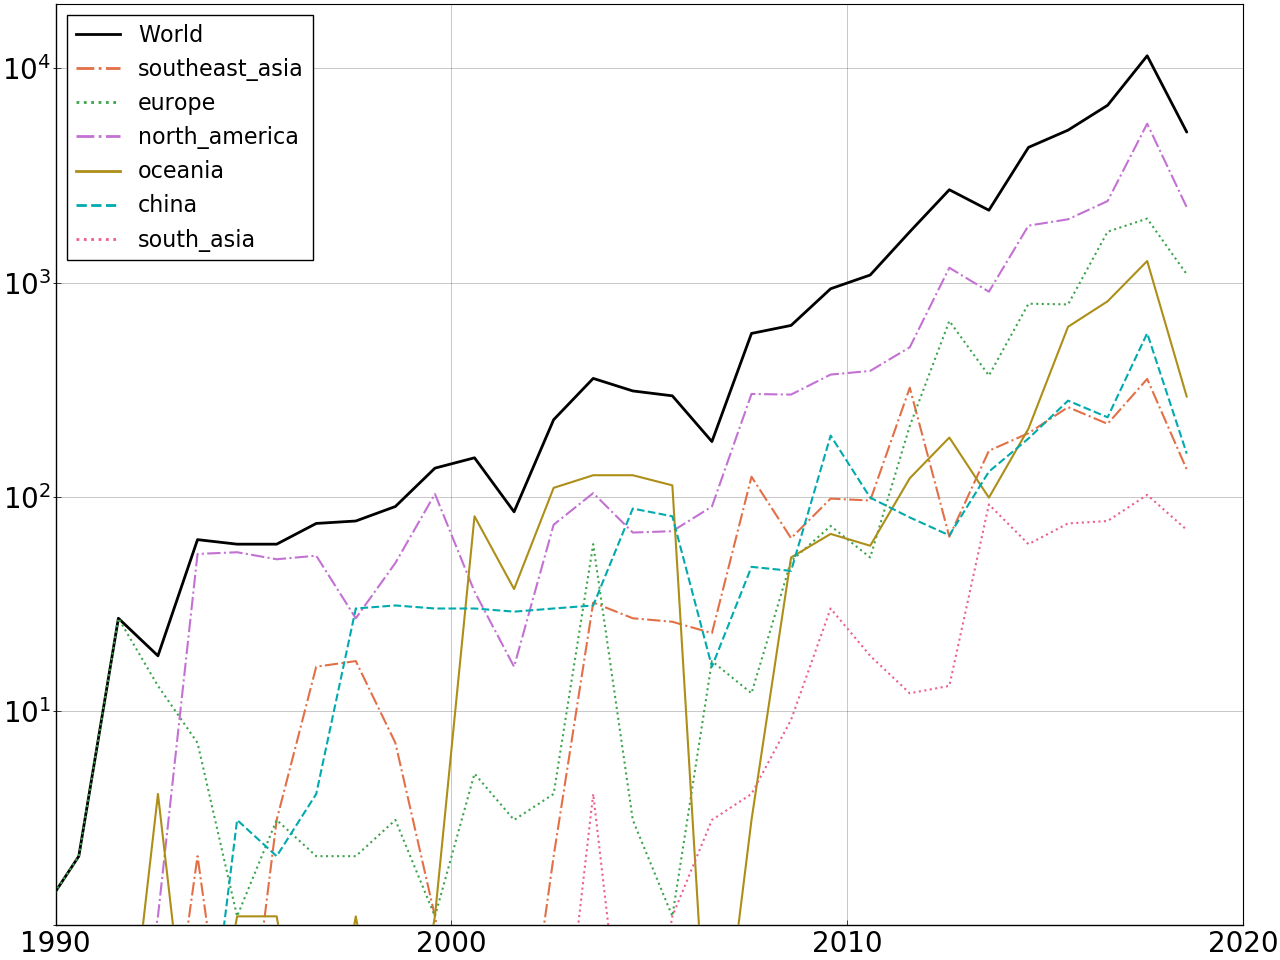
\includegraphics[scale=0.5]{SM_figures/Nseq_per_year.png}
		\caption{Supplementary figure 1 - Number of HA sequences per year from year 1990. }
		\label{fig:nseq_per_year}
	\end{figure}
	\begin{figure}
		\centering
		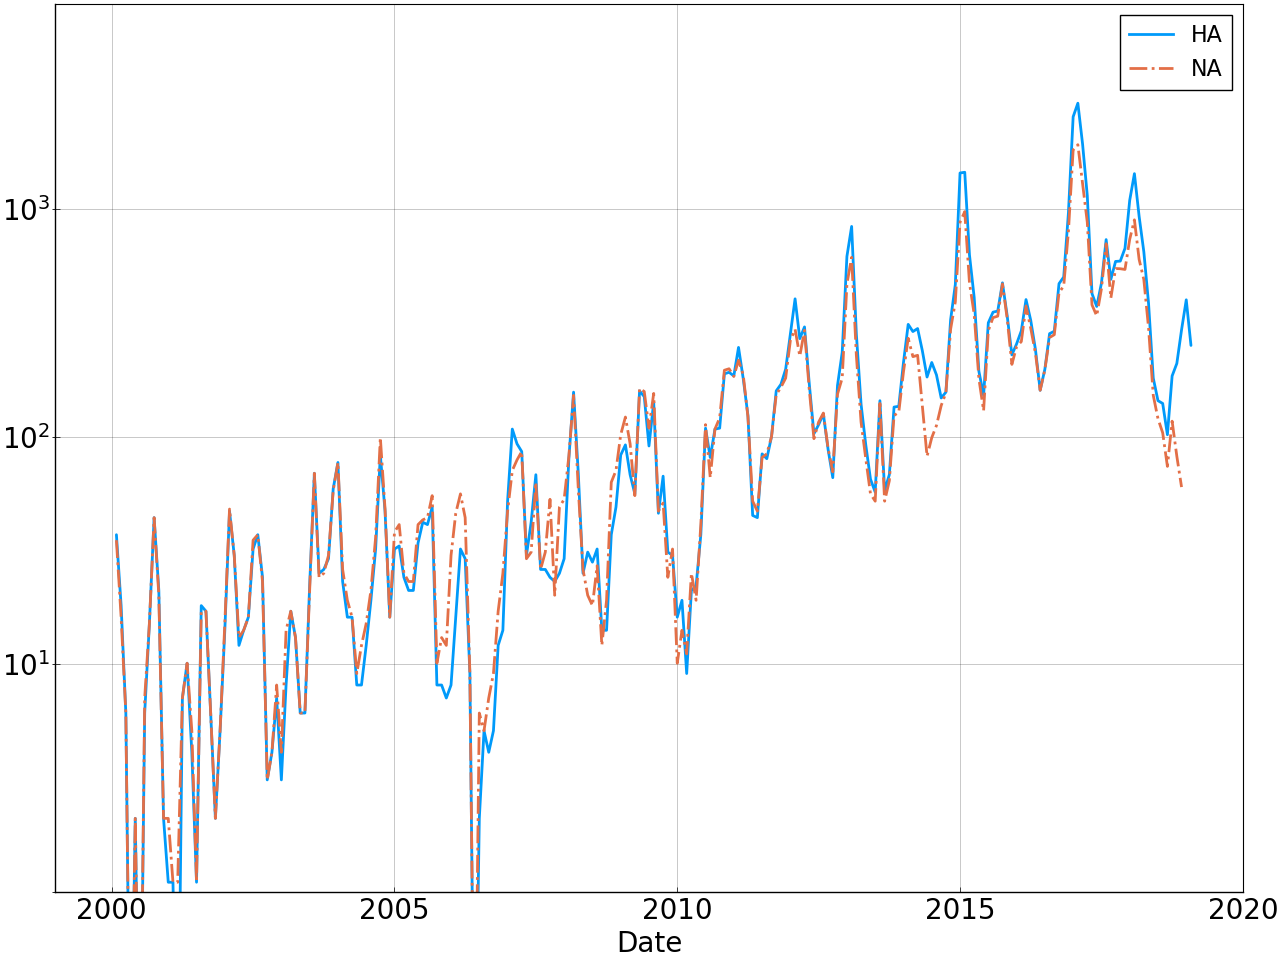
\includegraphics[scale=0.5]{Figures/Nseq_per_month.png}
		\caption{Supplementary figure 2 - Number of HA sequences per month from year 2000. }
		\label{fig:nseq_per_month}
	\end{figure}

	\begin{figure}
		\centering
		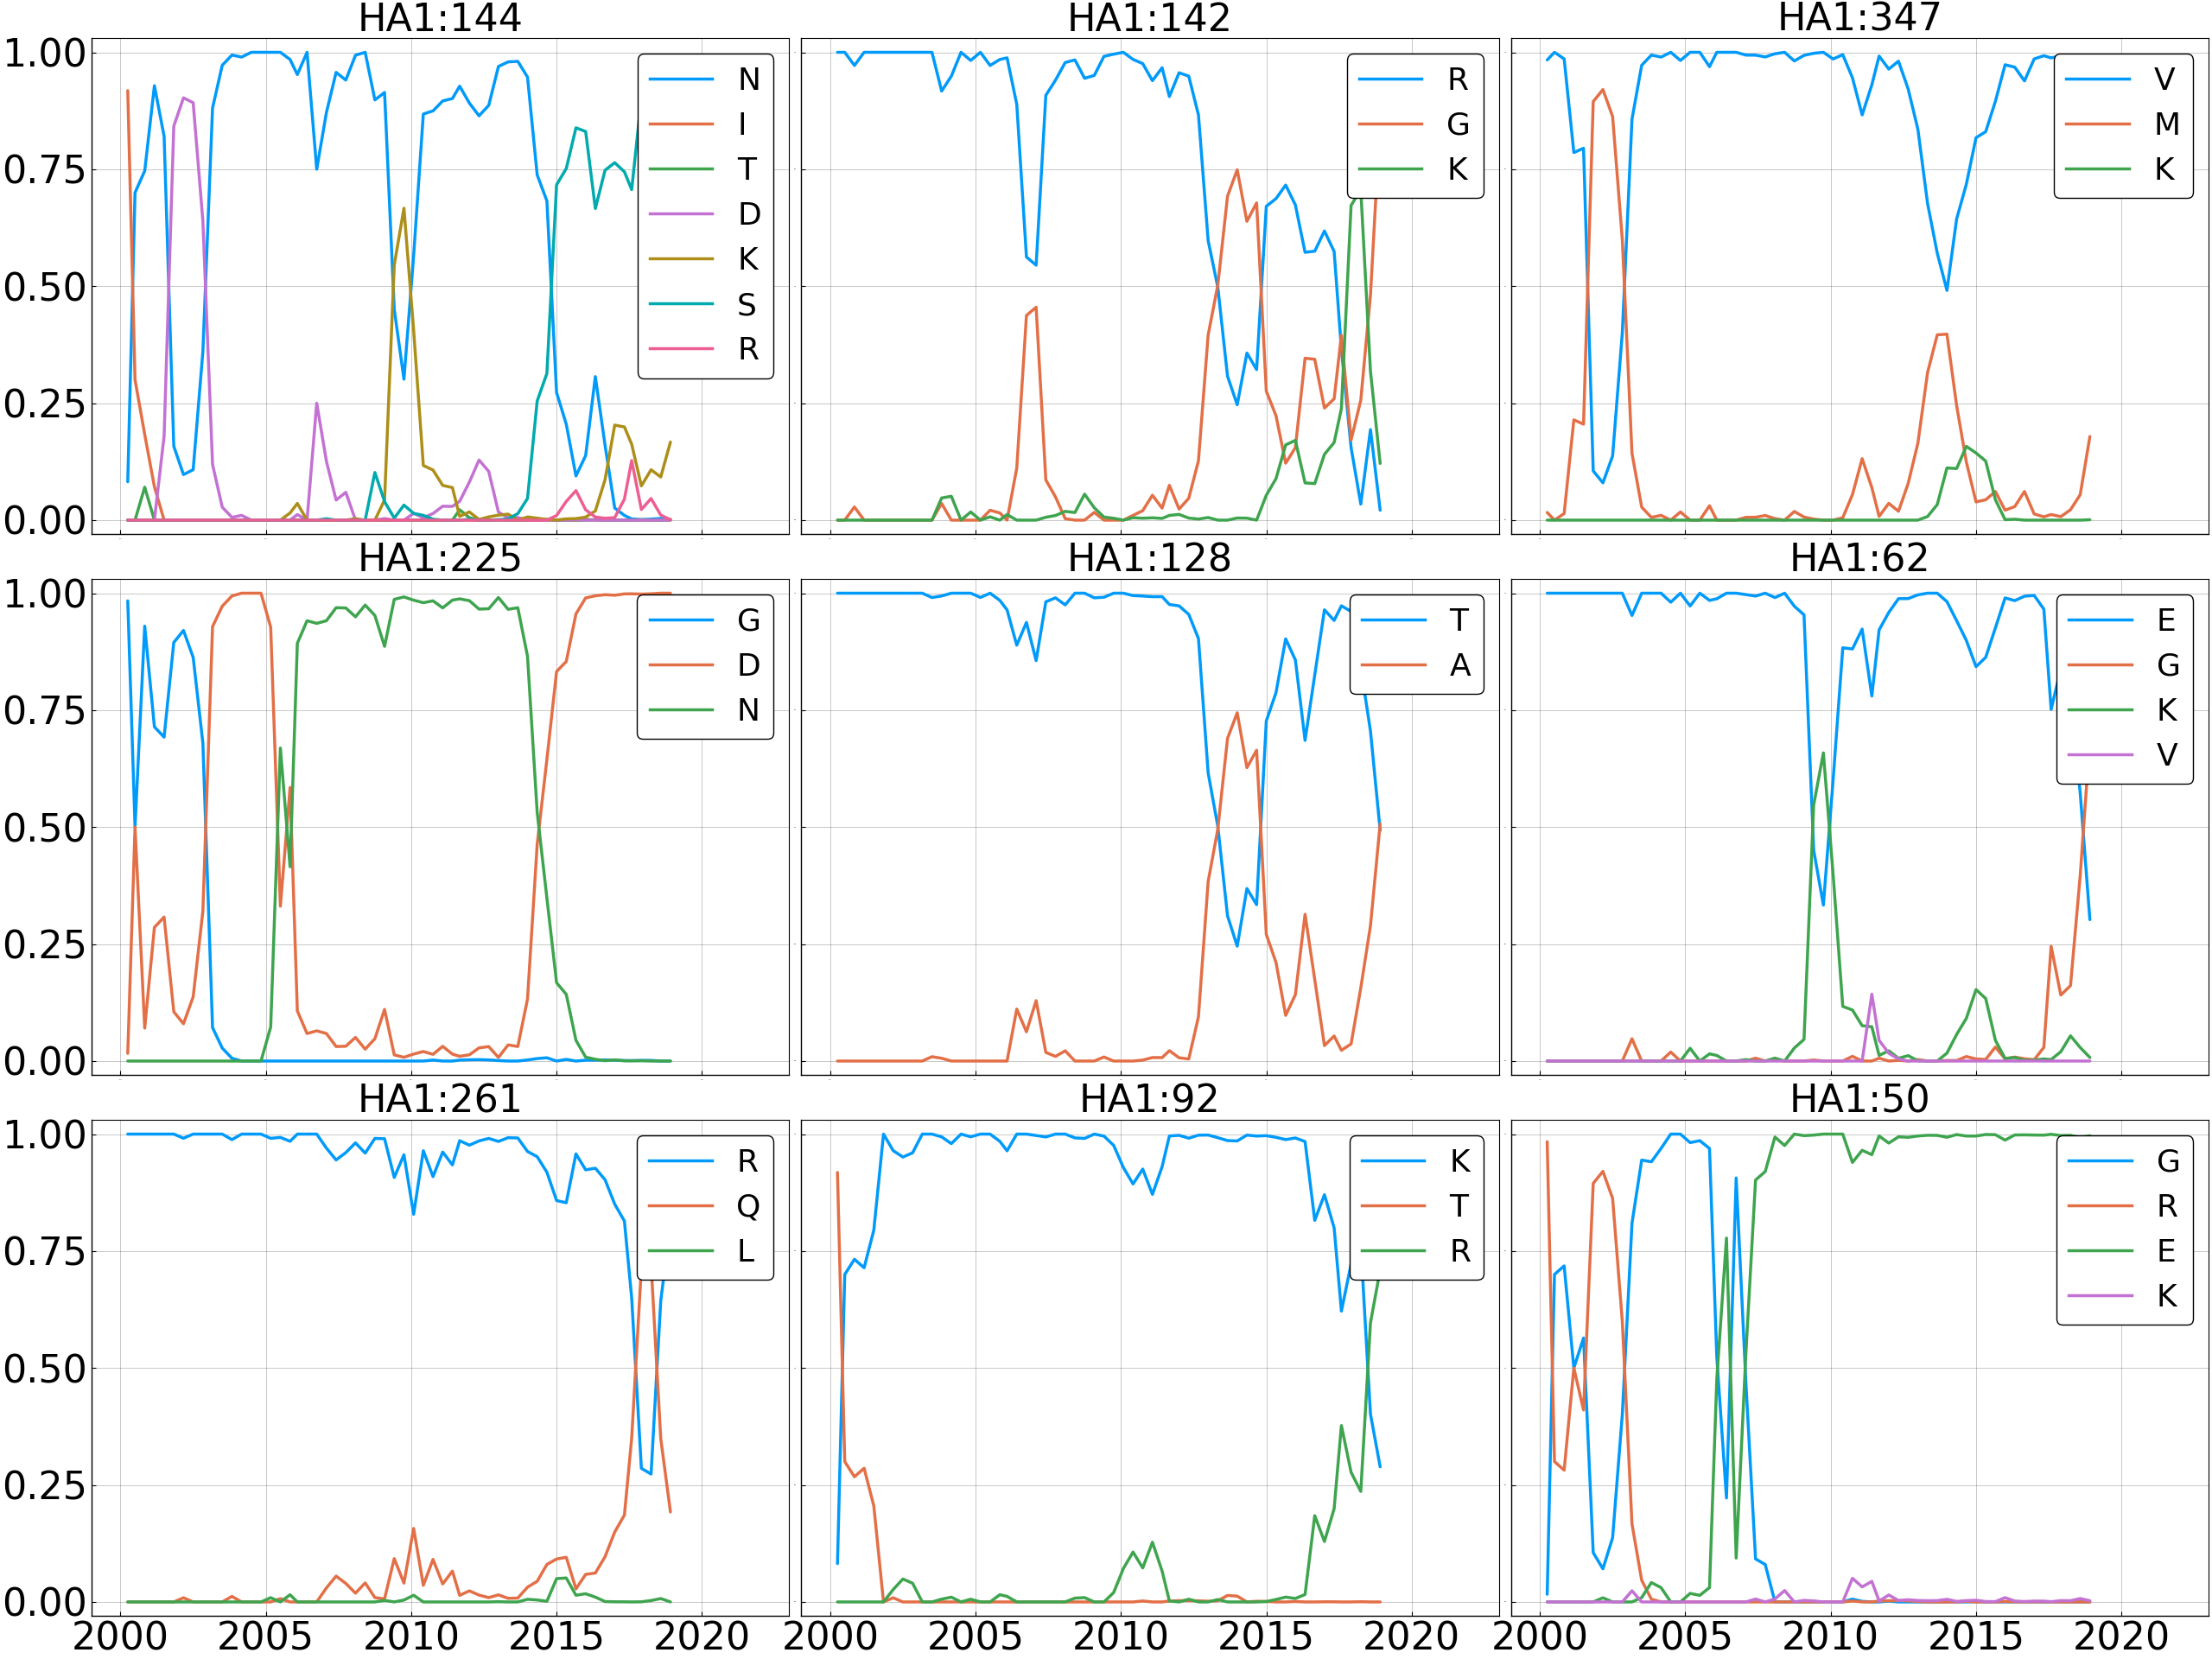
\includegraphics[scale=0.25]{Figures/sample_trajectories.png}
		\caption{Supplementary figure 3 - Frequency trajectories for the 9 most entropic positions in the HA protein.}
		\label{fig:sample_trajectories}
	\end{figure}

	% \begin{figure}
	% 	\centering
	% 	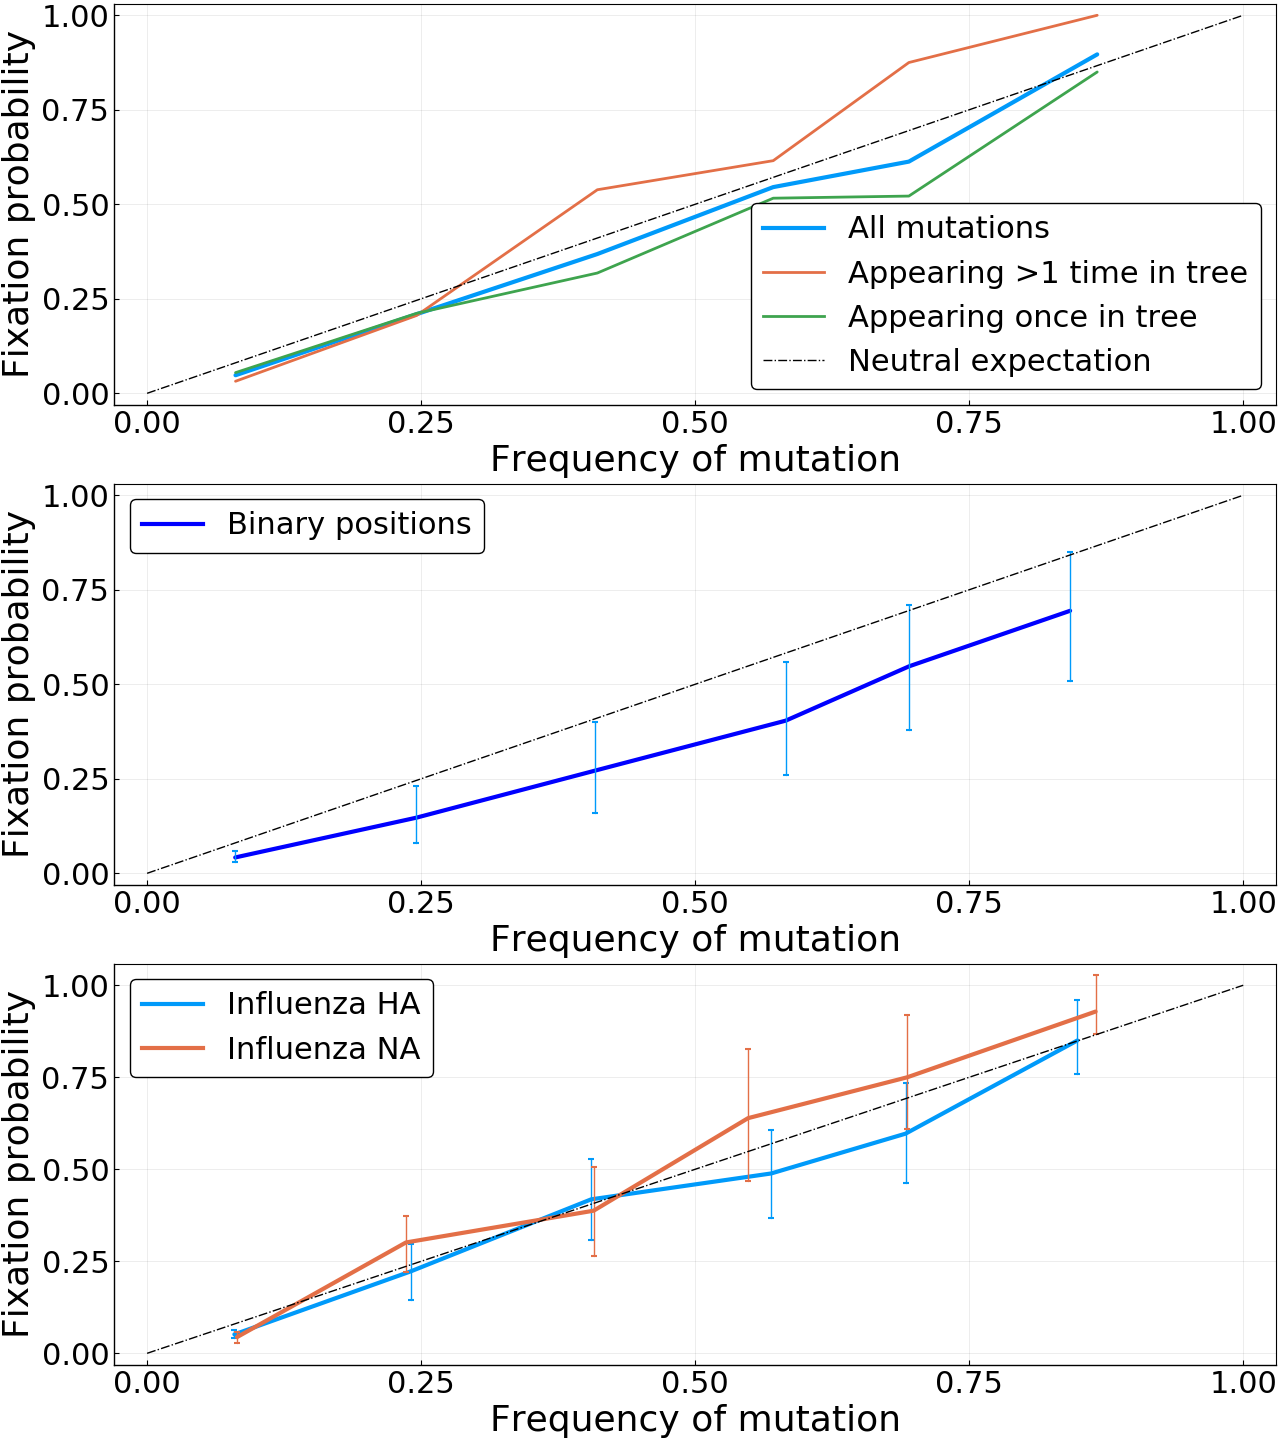
\includegraphics[width=0.9\textwidth]{SM_figures/Pfix_v_freq_misc.png}
	% 	\caption{Supplementary figure 4 - Probability of a mutation to fix as a function of the frequency at which it is measured in the population, for the HA protein and for different types of mutations. \textbf{Top panel}: Number of times the mutation appears in the phylogenetic tree. \textbf{Middle panel}: Binary positions, \emph{i.e.} positions at which only 2 amino acids are ever observed at the same time. \textbf{Bottom panel}: Trajectories with a positive derivative when measured at frequency $f$.}
	% 	\label{fig:pfix_v_freq_misc}
	% \end{figure}
	\begin{figure}
		\centering
		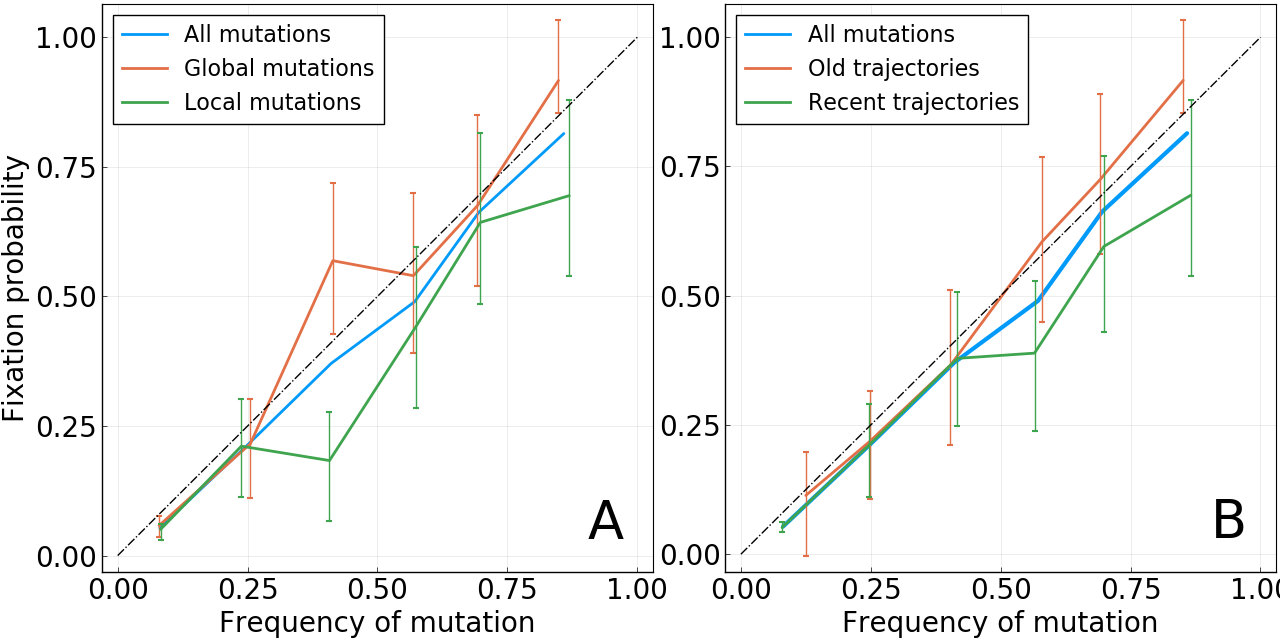
\includegraphics[width=0.9\textwidth]{SM_figures/geospread_and_time.png}
		\caption{Supplementary figure 4 - \textbf{A}: Mutations with a higher or lower geographical spread, based on the median value of the score used (see Methods). \textbf{B}: Mutations whose trajectories are older or more recent, based on the median age of trajectories when reaching the considered frequency $f$.}
		\label{fig:geospread_and_time}
	\end{figure}

	\begin{figure}
		\centering
		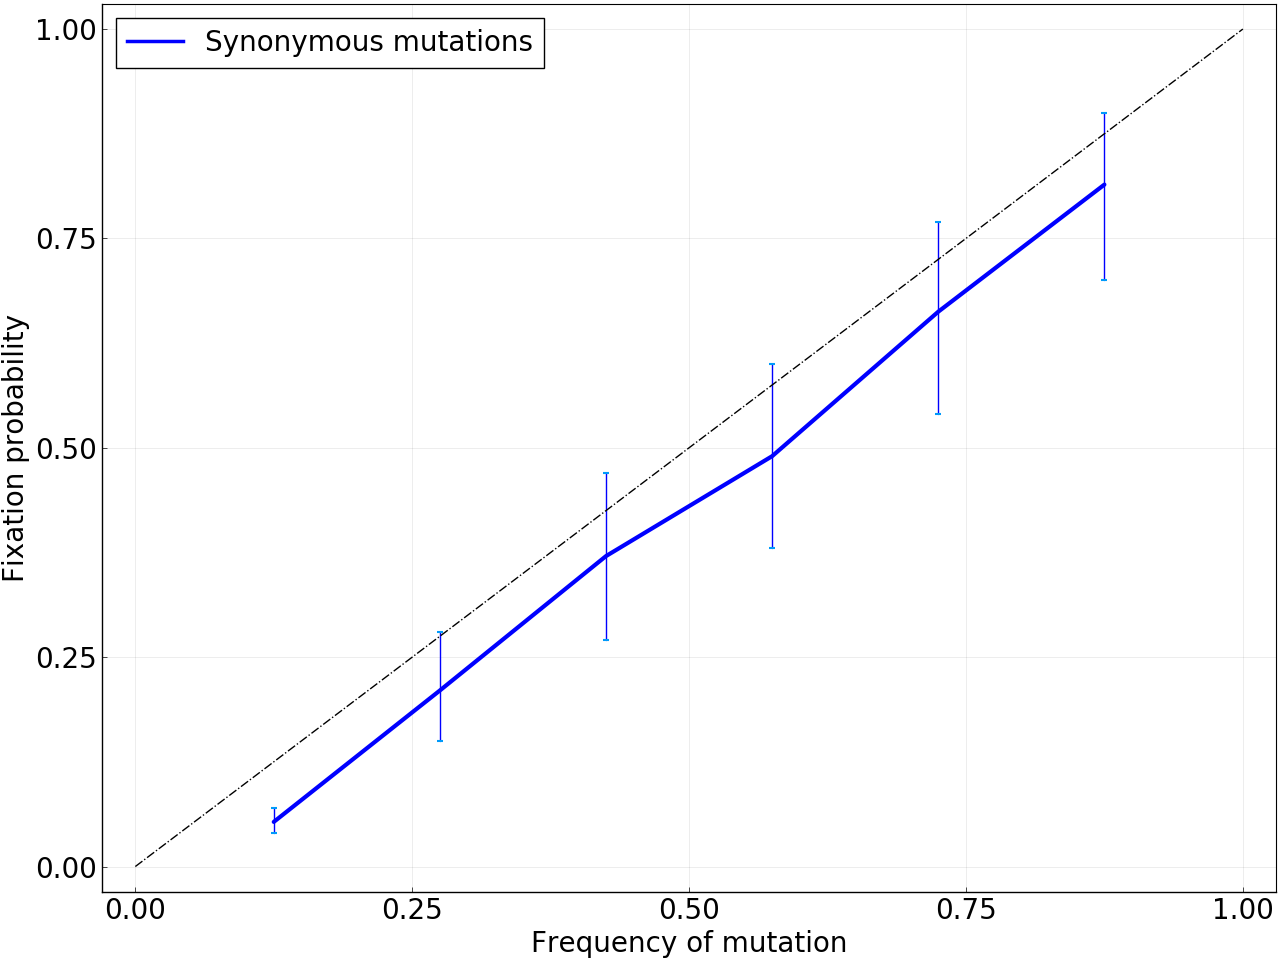
\includegraphics[width=0.9\textwidth]{SM_figures/Pfix_v_freq_syn.png}
		\caption{Supplementary figure 5 - Probability of a mutation to fix as a function of the frequency at which it is measured in the population, for the HA protein and for synonymous mutations.}
		\label{fig:pfix_v_freq_syn}
	\end{figure}

	\begin{figure}
		\centering
		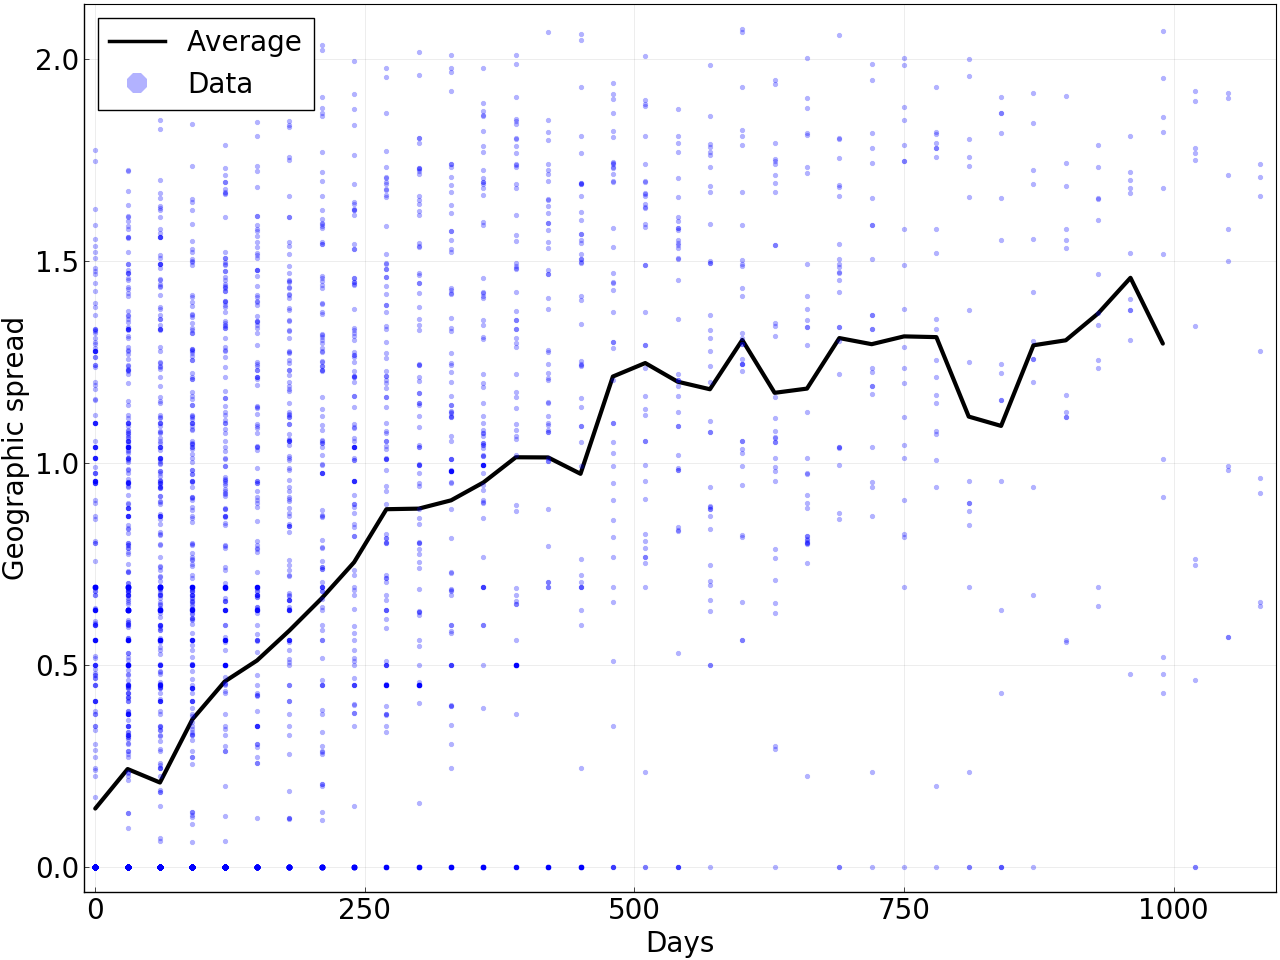
\includegraphics[width=0.9\textwidth]{SM_figures/GeoSpread_v_time_ha.png}
		\caption{Supplementary figure 6 - Geographic spread of mutations as a function of the time for which they have been present in the population above a frequency of 5\%. Points represent individual mutations and for a population in a given time bin. The line is the average of dots for a given value on the $x$-axis.}
		\label{fig:geospread_v_time}
	\end{figure}

	\begin{figure}
		\centering
		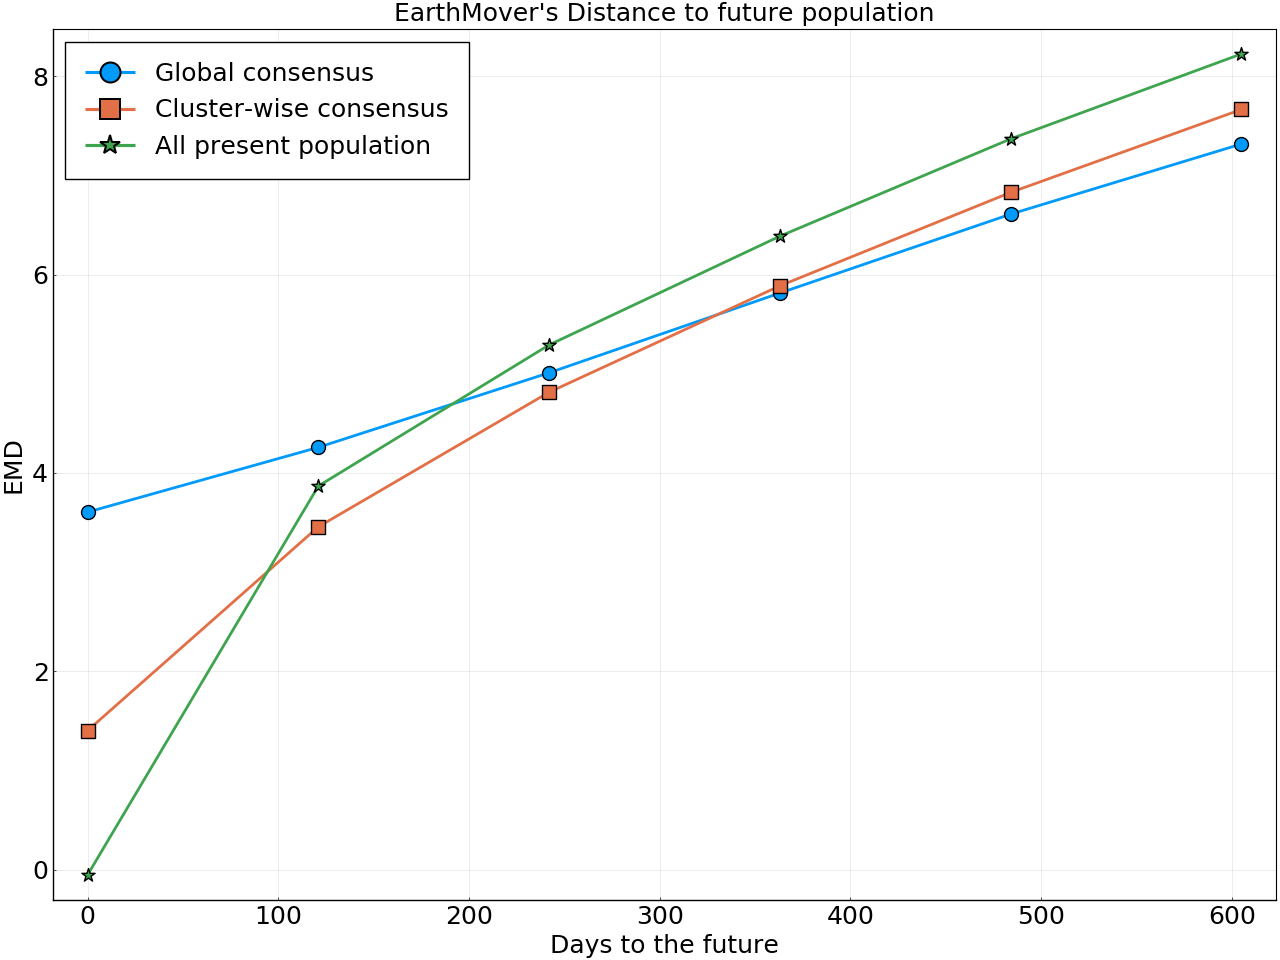
\includegraphics[width=0.9\textwidth]{SM_figures/EMD_to_future.png}
		\caption{Supplementary figure 7 - Earthmover's distance to the future population for different predictors. A present population consists of all HA sequences sampled in a 4 months time window. Quantities are averaged over all possible "present" populations from the year 2002. Predictors are: \textbf{Global consensus}: Consensus sequence of the present population. Best long-term predictor for a structure-less neutrally evolving population. \textbf{All present population}: All sequences in the present population. Perfect predictor if the population does not change at all through time. \textbf{Cluster-wise consensus}: Consensus sequence for each cluster in the present population. Clusters are based on maxima of the LBI. Sequences are assigned to a given cluster based on their tree distance to the corresponding local maximum.}
		\label{fig:emd_to_future}
	\end{figure}

	\begin{figure}
		\centering
		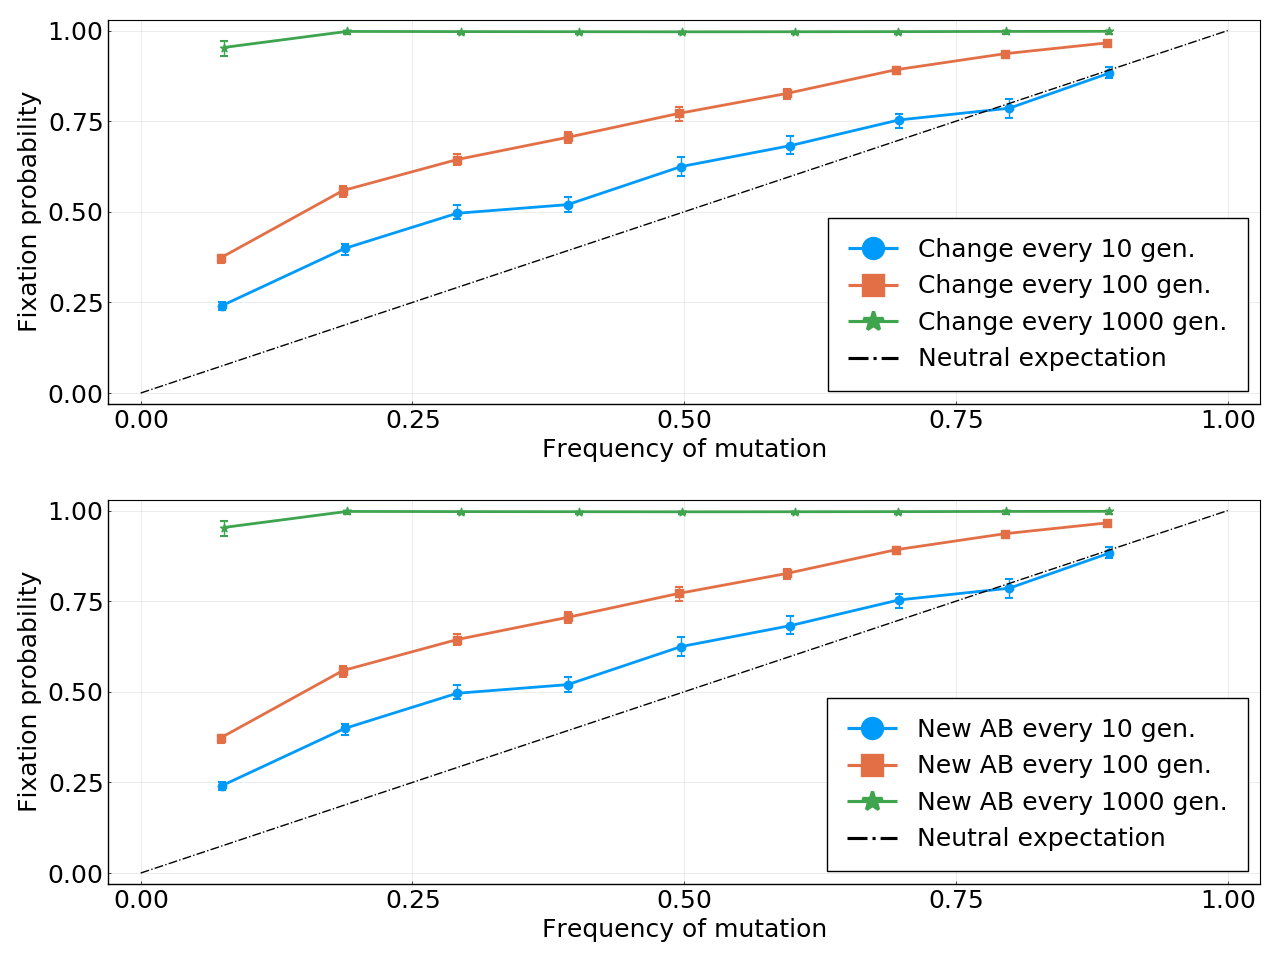
\includegraphics[width=0.9\textwidth]{SM_figures/simulation.png}
		\caption{Supplementary figure 8 - Simulations}
		\label{fig:simulations}
	\end{figure}


% subsection supplementary_figures (end)

% section supplementary_material (end)


\end{document}